\documentclass[12pt,a4paper]{report}

% ==============================================================================
% JKUAT UPRO PROJECT REPORT
% ==============================================================================

\usepackage[T1]{fontenc}
\usepackage{graphicx}
\usepackage{amsmath,amssymb}
\usepackage{geometry}
\usepackage{pgfgantt}
\usepackage{setspace}
\usepackage{cite}
\usepackage{hyperref}
\usepackage{titlesec}
\usepackage{caption}
\usepackage{listings}
\usepackage{booktabs}
\usepackage{xcolor}
\usepackage{tikz}
\usepackage{array}
\usepackage{tabularx}
\usepackage{longtable}
\usepackage{float}
\usepackage{multirow}
\usepackage{enumitem}

\usetikzlibrary{
    arrows,
    arrows.meta,
    calc,
    fit,
    positioning,
    shapes.geometric,
    shapes.multipart
}

\definecolor{nemoblue}{HTML}{1D4ED8}
\definecolor{nemoteal}{HTML}{0F766E}
\definecolor{nemoorange}{HTML}{B45309}
\definecolor{nemogray}{HTML}{475569}
\definecolor{nemolight}{HTML}{EFF6FF}
\definecolor{passgreen}{HTML}{166534}
\definecolor{warningred}{HTML}{991B1B}

% TikZ styles based on the report template.
\tikzstyle{startstop}=[
    rectangle,
    rounded corners,
    minimum width=3cm,
    minimum height=1cm,
    align=center,
    draw=nemoblue,
    fill=nemolight,
    thick
]
\tikzstyle{process}=[
    rectangle,
    rounded corners,
    minimum width=3cm,
    minimum height=1cm,
    align=center,
    draw=nemoblue,
    fill=nemolight,
    thick
]
\tikzstyle{decision}=[
    diamond,
    aspect=2,
    minimum width=3cm,
    minimum height=1cm,
    align=center,
    draw=nemoblue,
    fill=nemolight,
    thick
]
\tikzstyle{arrow}=[thick,->,>=stealth,draw=nemoblue]

\lstdefinestyle{nemo}{
    basicstyle=\ttfamily\footnotesize,
    breaklines=true,
    frame=single,
    keywordstyle=\color{nemoblue}\bfseries,
    stringstyle=\color{nemoorange},
    commentstyle=\color{passgreen},
    showstringspaces=false,
    numbers=left,
    numberstyle=\tiny\color{nemogray},
    captionpos=b,
    columns=fullflexible
}
\lstset{style=nemo}

\geometry{
    top=2cm,
    bottom=2.5cm,
    left=1in,
    right=1in
}
\onehalfspacing
\setlength{\parindent}{1.25cm}
\setlength{\parskip}{0pt}
\setlist{itemsep=0.25em,topsep=0.4em}
\emergencystretch=2em

\hypersetup{
    colorlinks=true,
    linkcolor=black,
    filecolor=black,
    urlcolor=black,
    citecolor=black,
    plainpages=false,
    pdftitle={Development and Evaluation of an Auditable, Resource-Conscious Parametric Optimization Workflow for Marine Structural Components},
    pdfauthor={Amina Ahmed Bwana and Mboje Abdullah}
}

\captionsetup{
    font=small,
    labelfont=bf,
    justification=centering,
    singlelinecheck=false
}
\captionsetup[table]{position=top}

\newcommand{\NEMO}{\textsc{Nemo}}
\newcommand{\code}[1]{\texttt{#1}}
\newcommand{\screeningwarning}{%
    \textit{The values in this section are first-order screening estimates.
    They are not certified engineering results and do not establish
    manufacturing or service suitability.}%
}

\begin{document}

\title{Development and Evaluation of an Auditable, Resource-Conscious
Parametric Optimization Workflow for Marine Structural Components}
\author{Amina Ahmed Bwana \and Mboje Abdullah}
\date{2026}

% ==============================================================================
% FRONT MATTER
% ==============================================================================

\hypersetup{pageanchor=false}
\begin{titlepage}
\thispagestyle{empty}
\begin{center}
{\setstretch{1.0}

\vspace*{0.2cm}


\includegraphics[width=0.20\textwidth]{./media/HDlogo.png}\\[0.45cm]

JOMO KENYATTA UNIVERSITY\\[0.2cm]
OF\\[0.2cm]
AGRICULTURE AND TECHNOLOGY\\[0.35cm]

COLLEGE OF ENGINEERING AND TECHNOLOGY\\[0.35cm]

SCHOOL OF MECHANICAL, MANUFACTURING AND MATERIALS ENGINEERING\\[0.35cm]

DEPARTMENT OF MARINE ENGINEERING AND MARITIME OPERATIONS\\[0.35cm]

BACHELOR OF SCIENCE IN MARINE ENGINEERING

\vspace{0.55cm}
\hrule
\vspace{0.3cm}

{\large\bfseries
DEVELOPMENT AND EVALUATION OF AN AUDITABLE,\\[0.08cm]
RESOURCE-CONSCIOUS PARAMETRIC OPTIMIZATION\\[0.08cm]
WORKFLOW FOR MARINE STRUCTURAL COMPONENTS}

\vspace{0.3cm}
\hrule

\vspace{0.5cm}

{\normalsize\textbf{MR-PRO-26-XX}}\\[0.25cm]

{\normalsize by}\\[0.2cm]
{\large\textbf{AMINA AHMED BWANA - ENM241-0087/2022}}\\[0.05cm]

{\large\textbf{MBOJE ABDULLAH - ENM241-0088/2022}}\\[0.05cm]

{\normalsize Supervised by}\\[0.15cm]
{\large\textbf{SUPERVISOR NAME}}

\vfill

{\footnotesize\textit{A project report submitted in partial fulfilment of the requirements}}\\
{\footnotesize\textit{for the award of the Degree of Bachelor of Science in Marine Engineering}}\\
{\footnotesize\textit{at the Jomo Kenyatta University of Agriculture and Technology}}\\[0.2cm]

{\footnotesize March 2027}
}
\end{center}
\end{titlepage}
\hypersetup{pageanchor=true}

\pagenumbering{roman}

\section*{DECLARATION}
\addcontentsline{toc}{section}{Declaration}

We hereby declare that this Project Report is our original work and has not
been presented for a degree in any other university or for any other award.

\vspace{1cm}
\noindent
\textbf{Name:} Amina Ahmed Bwana
\hfill
\textbf{REG NUMBER:} ENM241-0087/2022\\[0.5cm]
\noindent
\textbf{Signature:} \underline{\hspace{5cm}}
\hfill
\textbf{Date:} \underline{\hspace{4cm}}

\vspace{1cm}
\noindent
\textbf{Name:} Mboje Abdullah
\hfill
\textbf{REG NUMBER:} ENM241-0088/2022\\[0.5cm]
\noindent
\textbf{Signature:} \underline{\hspace{5cm}}
\hfill
\textbf{Date:} \underline{\hspace{4cm}}

\vspace{1cm}
\noindent
\textbf{Supervisor Declaration}

\noindent
This Project Report has been submitted for examination with my approval as
the University Supervisor.

\vspace{0.8cm}
\noindent
\textbf{Name:} Supervisor Name

\vspace{1cm}
\noindent
\textbf{Signature:} \underline{\hspace{5cm}}
\hfill
\textbf{Date:} \underline{\hspace{4cm}}

\clearpage

\chapter*{Dedication}
\addcontentsline{toc}{section}{Dedication}

We dedicate this Project Report to our parents, guardians, lecturers, and
mentors. Their encouragement, sacrifice, and guidance supported our academic
journey and the completion of this project.

\clearpage

\chapter*{Acknowledgements}
\addcontentsline{toc}{section}{Acknowledgements}

We thank our supervisor for the technical guidance, critical questions, and
academic direction provided throughout this project. We also thank the staff
of the Department of Marine Engineering and Maritime Operations for the
knowledge and facilities that supported this work. We are grateful to our
classmates, friends, and families for their practical help and encouragement.
Autodesk educational access and the open-source Python community made it
possible to complete the software work without direct project expenditure.

\clearpage

\chapter*{Abstract}
\addcontentsline{toc}{section}{Abstract}

This project developed and evaluated the Nelder-Mead Marine Optimizer
(\NEMO), an auditable workflow for the parameterized mass optimization of
marine structural components. The system combines unit-aware engineering
definitions, first-order structural screening, seeded Latin-hypercube
sampling, bounded multi-start Nelder--Mead search, traceable run records, a
file-based Autodesk Fusion bridge, native CAD generation, semantic boundary
metadata, validation-package generation, and a results dashboard. Three
component archetypes were studied: an Aluminum 6061-T6 equipment bracket, an
S275 steel lifting padeye, and an Aluminum 6061-T6 stabilizer fin. Each part
used 60 seeded Latin-hypercube samples and three local-search starts. The
lightest selected analytically feasible finalists had masses of
0.1134~kg, 3.5478~kg, and 14.3154~kg, which corresponded to reductions of
72.9\%, 59.9\%, and 27.2\% from the respective analytical baselines. Native
Fusion CAD mass differed from the analytical estimate by 1.15\%, 3.80\%, and
0.59\% for these finalists. Generator sweeps tested each baseline and 20
seeded design vectors. The bracket and padeye completed all 21 integration
cases. The stabilizer generated all 21 artifacts, although the outer test
process reached its 30-minute timeout while reading the final response.
The bracket also preserved the proof-of-concept path into two exploratory
Fusion Static Stress studies. Their images identify the geometry, support and
load regions, and qualitative response patterns. The second study, however,
used 1.472~N instead of the intended 1472~N, while the first did not provide a
complete traceable load definition. Their numerical results were therefore
rejected. The work shows that a resource-conscious, human-reviewed workflow
can reduce routine search and CAD effort while keeping analytical, CAD, and
FEA claims separate. The reported designs remain screening candidates. They
require corrected, mesh-converged FEA, design-code checks, verified loads and
materials, fatigue and fabrication assessment, and qualified engineering
review before manufacture or service.

\clearpage
\tableofcontents
\clearpage
\listoffigures
\clearpage
\listoftables
\clearpage

\section*{LIST OF ABBREVIATIONS AND SYMBOLS}
\addcontentsline{toc}{section}{List of Abbreviations and Symbols}

\subsection*{Abbreviations}
\begin{longtable}{p{0.22\textwidth}p{0.68\textwidth}}
\textbf{API} & Application Programming Interface\\
\textbf{CAD} & Computer-Aided Design\\
\textbf{CAE} & Computer-Aided Engineering\\
\textbf{CFD} & Computational Fluid Dynamics\\
\textbf{CLI} & Command-Line Interface\\
\textbf{FEA} & Finite Element Analysis\\
\textbf{FOS} & Factor of Safety\\
\textbf{IPC} & Inter-Process Communication\\
\textbf{JSON} & JavaScript Object Notation\\
\textbf{JKUAT} & Jomo Kenyatta University of Agriculture and Technology\\
\textbf{LHS} & Latin-Hypercube Sampling\\
\textbf{NACA} & National Advisory Committee for Aeronautics\\
\textbf{NEMO} & Nelder-Mead Marine Optimizer\\
\textbf{POC} & Proof of Concept\\
\textbf{SI} & International System of Units\\
\textbf{STEP} & Standard for the Exchange of Product Model Data\\
\textbf{STL} & Stereolithography mesh format\\
\textbf{V\&V} & Verification and Validation\\
\end{longtable}

\subsection*{Symbols}
\begin{longtable}{p{0.22\textwidth}p{0.68\textwidth}}
$A$ & Area (m$^2$)\\
$b$ & Stabilizer span (m)\\
$C_L$ & Lift coefficient\\
$E$ & Young's modulus (Pa)\\
$F_d$ & Design load (N)\\
$F_{\min}$ & Minimum permitted factor of safety\\
$g$ & Acceleration due to gravity (m/s$^2$)\\
$I$ & Second moment of area (m$^4$)\\
$J(\mathbf{x})$ & Penalized optimization objective\\
$K_t$ & Stress-concentration factor\\
$m$ & Mass (kg)\\
$M$ & Bending moment (N\,m)\\
$\rho$ & Density (kg/m$^3$)\\
$\sigma$ & Normal or equivalent stress (MPa)\\
$\sigma_y$ & Material yield strength (MPa)\\
$\tau$ & Shear stress (MPa)\\
$V$ & Volume (m$^3$) or speed (m/s), as identified in context\\
$w$ & Penalty weight\\
$\mathbf{x}$ & Physical design vector\\
$\mathbf{z}$ & Scaled design vector\\
$\delta$ & Displacement (mm)\\
$\delta_{\max}$ & Maximum permitted displacement (mm)\\
\end{longtable}

\clearpage

% ==============================================================================
% MAIN CONTENT
% ==============================================================================

\pagenumbering{arabic}
\label{page:main-start}

\chapter{Introduction}
\label{chap:introduction}

Marine vessels contain numerous brackets, foundations, lifting fittings, and control-surface structures. These components must transmit demanding loads without yielding or excessive deformation while contributing as little unnecessary mass as practicable. Excess mass increases material consumption and vessel displacement, whereas excessive material removal reduces stiffness and fatigue resistance. Marine structural design is therefore a constrained engineering problem.

\section{Problem Statement}
Conventional component design uses hand calculations, conservative initial sizing, CAD modelling, and repeated checks. Only a limited number of dimensional combinations can normally be examined manually. A systematic method was required to explore plate dimensions, stiffener sizes, and fillet radii while enforcing strength and deflection limits.

\section{Objectives}
The main objective was to develop and assess a parameterized engineering method for lower-mass marine structural components. The specific objectives were to:
\begin{enumerate}
\item define materials, loads, boundary conditions, variables, and acceptance criteria;
\item formulate analytical models for mass, stress, factor of safety, and deflection;
\item explore the bracket design space by Latin-hypercube sampling and bounded Nelder--Mead optimization;
\item generate parameterized geometry and validation candidates in Fusion 360;
\item extend the method to a lifting padeye and fixed-envelope stabilizer fin; and
\item identify the detailed FEA and physical validation required before practical adoption.
\end{enumerate}

\section{Scope and Significance}
Completed work covered linear-elastic analytical screening, continuous dimensional variables, CAD generation, and validation preparation. Fatigue, buckling, weld-detail stress, corrosion, nonlinear contact, vibration, impact, CFD, fabrication, and proof testing were outside the completed scope. The engineering value lies in traceable comparison of alternatives, not in replacing detailed analysis or professional judgement.

\chapter{Literature Review}
\label{chap:literature}

This chapter reviews the established methods on which \NEMO\ is based. The
review covers constrained structural optimization, derivative-free search,
Nelder--Mead, variable scaling, Latin-hypercube sampling, tiered model
fidelity, CAD--CAE integration, simulation intent, marine structural
applications, and computational-model credibility. It then relates these
topics to the bracket, padeye, and stabilizer case studies and defines the
limited research gap addressed by this project.

\section{Structural Optimization Methods}
\label{sec:structural-optimization}

\subsection{Constrained Search}

Structural optimization formalizes the selection of design variables to
improve an objective while satisfying constraints. An objective can represent
mass, cost, compliance, displacement, stress, fatigue damage, environmental
impact, or a weighted combination of measures. Constraints can represent
strength, stiffness, stability, vibration, geometry, fabrication, inspection,
or regulatory limits. The problem is written in the general form

\begin{align}
\underset{\mathbf{x}}{\text{minimize}}\quad
    & f(\mathbf{x}), \label{eq:general-objective}\\
\text{subject to}\quad
    & g_j(\mathbf{x})\leq 0,\quad j=1,\ldots,m,\\
    & h_k(\mathbf{x})=0,\quad k=1,\ldots,p,\\
    & \mathbf{l}\leq\mathbf{x}\leq\mathbf{u},
\end{align}

where $\mathbf{x}$ is the design vector, $f$ is the objective, $g_j$ and
$h_k$ are inequality and equality constraints, and $\mathbf{l}$ and
$\mathbf{u}$ are variable bounds.

Structural optimization is commonly divided into size, shape, and topology
optimization. Size optimization changes dimensions such as thickness and
section area. Shape optimization changes geometric boundaries while retaining
a general feature arrangement. Topology optimization changes the distribution
or connectivity of material inside a design region. These classes can overlap,
but the distinction helps define what an optimization claim means.

\NEMO\ performs size and bounded parametric shape optimization. The number and
general arrangement of major features remain fixed. The optimizer changes
dimensions such as plate thickness, rib height, lug width, spar position, and
fillet radius. It does not remove arbitrary material or create a new topology.
This restriction keeps every candidate compatible with an intended load path,
a native CAD generator, and predefined load and support roles.

The project uses mass as the principal objective. This choice is easy to
measure and compare, but it does not make mass the only design criterion. A
low-mass candidate is useful only if its constraints pass and its omitted
failure modes are later checked. In marine practice, this qualification is
especially important because cyclic loading, corrosion, fabrication detail,
and uncertain operational loads can govern a design that passes one static
yield check.

\subsection{Derivative-Free Optimization}
\label{sec:derivative-free}

Many engineering analyses appear as black-box functions to the optimizer. The
optimizer supplies dimensions and receives calculated outputs, but it does not
have exact derivatives of those outputs. CAD regeneration, meshing changes,
solver tolerances, discrete feature behavior, and failed candidates can also
make numerical gradients unreliable.

Direct-search and derivative-free methods use objective values without
requiring analytical gradients. Kolda, Lewis, and Torczon reviewed the
development of direct-search methods and distinguished methods with formal
convergence properties from more heuristic searches \cite{kolda2003}. Their
review shows that derivative-free operation is not the same as assumption-free
operation. The designer must still scale variables, handle bounds, define
constraints, select termination criteria, and evaluate sensitivity to the
starting point.

Derivative-free methods can be attractive when each function evaluation is
moderately expensive and the number of variables is limited. They are less
attractive when the dimension is very high or when gradients can be calculated
cheaply and reliably. The three \NEMO\ cases contain six or nine continuous
variables. Their analytical evaluations are inexpensive, while the wider
workflow includes potential discontinuities from geometry checks. This
combination supports the use of a simple derivative-free method for the
reference implementation.

\subsection{The Nelder--Mead Simplex Method}
\label{sec:nelder-mead-review}

Nelder and Mead introduced the simplex method in 1965 \cite{nelder1965}. In an
$n$-dimensional space, the method maintains $n+1$ vertices. It evaluates and
ranks these vertices, calculates the centroid of the better vertices, and
attempts to replace the worst vertex. The standard trial operations are
reflection, expansion, contraction, and shrink.

If $\mathbf{x}_h$ is the worst vertex and $\bar{\mathbf{x}}$ is the centroid
of the remaining vertices, a reflected point is

\begin{equation}
\mathbf{x}_r=\bar{\mathbf{x}}+
\alpha(\bar{\mathbf{x}}-\mathbf{x}_h),
\label{eq:nm-reflection}
\end{equation}

where $\alpha$ is the reflection coefficient. A sufficiently good reflection
can lead to expansion:

\begin{equation}
\mathbf{x}_e=\bar{\mathbf{x}}+
\gamma(\mathbf{x}_r-\bar{\mathbf{x}}).
\label{eq:nm-expansion}
\end{equation}

An unsuccessful reflection can cause contraction toward the centroid. When
contraction also fails, the simplex shrinks toward its best vertex. The
standard coefficients used by \NEMO\ are $\alpha=1$, $\gamma=2$, $\rho=0.5$,
and $\sigma=0.5$.

The method has several practical advantages. It is compact, does not require a
gradient, and is easy to explain and implement. It also has important limits.
Lagarias \emph{et al.} established convergence results under restricted
conditions and discussed cases where the method can approach a non-minimizer
\cite{lagarias1998}. Nelder--Mead is a local search. Its final design can
depend on the initial simplex, variable scaling, bounds, penalties, and the
shape of the objective landscape.

These limitations affect the language of this report. One local run cannot
support a claim of global optimality. \NEMO\ uses a seeded design-space sample
and three starts to reduce dependence on the configured baseline. The report
uses the phrase ``best feasible design found within this parameterized
search.'' This wording is more defensible than ``global optimum.''

\begin{table}[H]
\centering
\caption{Nelder--Mead operations and their purpose in the implemented search}
\label{tab:nm-operations}
\begin{tabularx}{\textwidth}{p{0.18\textwidth}p{0.18\textwidth}X}
\toprule
\textbf{Operation} & \textbf{Coefficient} & \textbf{Purpose}\\
\midrule
Reflection & $\alpha=1$ & Tests a point across the centroid from the current
worst vertex.\\
Expansion & $\gamma=2$ & Extends a successful reflected step when it improves
the best objective.\\
Contraction & $\rho=0.5$ & Tests a shorter step when reflection does not give
adequate improvement.\\
Shrink & $\sigma=0.5$ & Moves all non-best vertices toward the best point after
failed trial steps.\\
\bottomrule
\end{tabularx}
\end{table}

\subsection{Variable Scaling, Bounds, and Constraint Penalties}
\label{sec:scaling-review}

Engineering variables can differ greatly in magnitude and unit. A plate
thickness may be 4~mm, a chordwise spar position may be 30\%, and a root
insert length may be 180~mm. If an optimizer works directly in these physical
coordinates, its simplex geometry and trial step sizes can be dominated by
the numerically largest variables.

\NEMO\ maps each physical variable $x_i$ to the scaled coordinate

\begin{equation}
z_i=\frac{x_i-l_i}{u_i-l_i},
\qquad 0\leq z_i\leq 1,
\label{eq:variable-scaling}
\end{equation}

where $l_i$ and $u_i$ are the lower and upper bounds. The evaluator performs
the inverse mapping before it uses the engineering equations. Trial points are
clipped at the scaled bounds.

Scaling gives each coordinate the same numerical range. It does not make the
physics equally sensitive. A small thickness change can alter both mass and
section properties strongly, while a similar scaled change in a fillet radius
may affect only one stress factor in the analytical model. Sensitivity remains
a property of the model.

Nelder--Mead does not directly enforce general nonlinear constraints in this
implementation. \NEMO\ therefore uses a penalty objective. If
$m(\mathbf{x})$ is mass, $F(\mathbf{x})$ is factor of safety,
$F_{\min}$ is the minimum factor of safety, $\delta(\mathbf{x})$ is
displacement, and $\delta_{\max}$ is the displacement limit, the objective is

\begin{equation}
\begin{split}
J(\mathbf{x})=m(\mathbf{x})+w\Bigg[
&\left(
\frac{\max(0,F_{\min}-F(\mathbf{x}))}{F_{\min}}
\right)^2\\
&+\left(
\frac{\max(0,\delta(\mathbf{x})-\delta_{\max})}
{\delta_{\max}}
\right)^2
\Bigg],
\end{split}
\label{eq:penalty-objective}
\end{equation}

with $w=100$ for the current parts.

A feasible design has $J=m$. An infeasible design has a higher objective
according to its normalized violations. Penalties simplify the search, but
their weight affects ranking. A weak penalty can make an infeasible light
design more attractive than a feasible heavier design. A large penalty can
create a steep landscape near the boundary. The final selection must therefore
filter explicitly for feasibility. The stabilizer case in
Chapter~\ref{chap:results} demonstrates why this check is necessary.

\subsection{Latin-Hypercube Sampling}
\label{sec:lhs-review}

McKay, Beckman, and Conover introduced Latin-hypercube sampling as a stratified
method for computer experiments \cite{mckay1979}. For each variable, an
$N$-point Latin hypercube samples once from each of $N$ equal-probability
intervals. Independent permutations combine the one-dimensional samples into
$N$ multi-dimensional points.

Compared with an unstructured random sample of the same size, a Latin
hypercube improves one-dimensional stratification. It does not guarantee dense
coverage of every interaction, especially in high dimensions. Sixty points
remain sparse in a nine-dimensional space. The method is therefore best
viewed here as an economical exploration step.

\NEMO\ uses 60 samples per part with seed 42. The fixed seed makes the
campaign repeatable. Sampling serves three purposes:

\begin{enumerate}
    \item it checks whether calculated outputs change in a physically sensible
    direction over the bounds;
    \item it identifies low-mass feasible candidates that can start local
    search; and
    \item it reduces reliance on one baseline-start Nelder--Mead run.
\end{enumerate}

Sampling also provides diagnostic evidence. A high failure rate can reveal
poor parameter bounds or a fragile geometry generator. An unexpectedly high
feasibility rate can reveal an over-conservative baseline or a screening model
that does not activate the declared constraints.

\section{Model Fidelity and CAD--CAE Integration}
\label{sec:model-fidelity-integration}

\subsection{Tiered Model Fidelity}
\label{sec:fidelity-review}

Engineering optimization often combines models with different cost and
accuracy. Peherstorfer, Willcox, and Gunzburger review multi-fidelity methods
that combine inexpensive low-fidelity models with expensive high-fidelity
models \cite{peherstorfer2018}. Formal multi-fidelity optimization uses the
high-fidelity model inside the optimization strategy to improve prediction,
selection, or convergence.

\NEMO\ does not yet implement such a closed loop. The analytical model guides
the search. Native CAD verifies geometry and mass for selected designs. Manual
FEA follows as a separate validation stage. The correct description is a
\emph{tiered-fidelity workflow}. The analytical optimum is not automatically
corrected by FEA.

\begin{figure}[H]
\centering
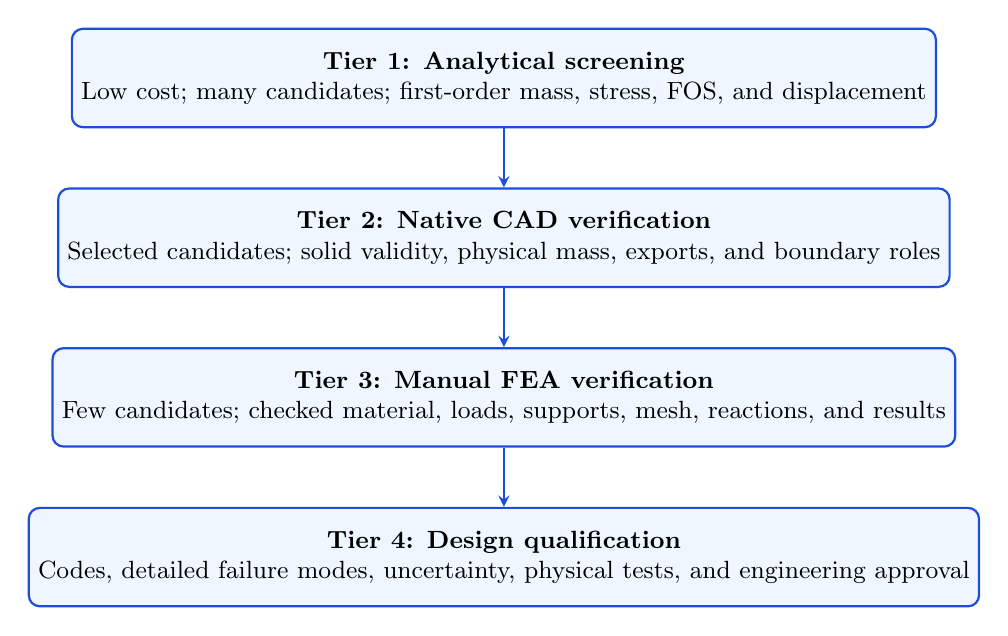
\begin{tikzpicture}[
    node distance=0.75cm,
    every node/.style={font=\small},
    stage/.style={
        rectangle,
        rounded corners,
        draw=nemoblue,
        fill=nemolight,
        thick,
        minimum width=0.83\textwidth,
        minimum height=1.25cm,
        align=center
    }
]
\node[stage] (a) {\textbf{Tier 1: Analytical screening}\\
Low cost; many candidates; first-order mass, stress, FOS, and displacement};
\node[stage,below=of a] (b) {\textbf{Tier 2: Native CAD verification}\\
Selected candidates; solid validity, physical mass, exports, and boundary roles};
\node[stage,below=of b] (c) {\textbf{Tier 3: Manual FEA verification}\\
Few candidates; checked material, loads, supports, mesh, reactions, and results};
\node[stage,below=of c] (d) {\textbf{Tier 4: Design qualification}\\
Codes, detailed failure modes, uncertainty, physical tests, and engineering approval};
\draw[arrow] (a) -- (b);
\draw[arrow] (b) -- (c);
\draw[arrow] (c) -- (d);
\end{tikzpicture}
\caption{Tiered evidence model used by the project}
\label{fig:tiered-evidence}
\end{figure}

The distinction between the tiers protects the report from a common error:
treating agreement on one quantity as complete validation. Close agreement
between analytical and CAD mass shows that the volume approximations represent
the generated geometry reasonably well. It does not show that the analytical
stress model represents local three-dimensional stress.

\subsection{CAD--CAE Integration}
\label{sec:cad-cae-review}

Automated structural optimization requires dependable communication between
geometry, analysis, and optimization. Park and Dang coupled commercial CAD and
CAE software through scripting, programming interfaces, and metamodels
\cite{park2010}. Their work shows how integration can reduce repetitive work
and analysis cost. It also introduces an additional source of error when a
surrogate model approximates the high-fidelity response.

Li \emph{et al.} developed a unified parametric representation based on
extended voxels. Their method supports a closed loop among design, simulation,
and optimization while carrying design and simulation meaning
\cite{li2023}. This work confirms that automated CAD--CAE optimization is an
established research area. \NEMO\ does not claim novelty from automation
alone.

The project instead uses a modest file-based architecture. External Python
handles engineering definitions, optimization, run records, and validation
packages. Fusion handles native CAD and physical properties. Versioned JSON
files connect the two environments. This approach is slower than an in-process
call but has useful properties:

\begin{itemize}
    \item a request and response can be inspected with an ordinary text editor;
    \item the Fusion environment does not need third-party optimization
    packages;
    \item a failed request can preserve a controlled error record;
    \item the protocol can retain compatibility with the original bracket
    proof of concept; and
    \item the same external application can later support another CAD or FEA
    backend.
\end{itemize}

The architecture also has limits. A single shared request directory serializes
CAD work. Polling adds latency. Local file locking requires retry behavior.
The bridge cannot make an unavailable solver API available. These are accepted
trade-offs for an inspectable student-scale implementation.

\subsection{Simulation Intent and Semantic Boundary Roles}
\label{sec:simulation-intent}

Geometry changes can invalidate an analysis even when the regenerated solid
looks correct. A load attached to a low-level face identifier can disappear or
move after a feature changes the boundary representation. A reliable
parametric workflow must preserve why a region exists and how it is used.

Nolan \emph{et al.} define simulation intent as the high-level modeling and
idealization decisions required for fit-for-purpose analysis
\cite{nolan2015}. Their work associates analysis meaning with regions and
interfaces rather than relying only on unstable topology.

\NEMO\ applies the same principle in a smaller implementation. The bracket
declares \code{fixed\_support} and \code{equipment\_load}. The padeye declares
\code{fixed\_support} and \code{pin\_bearing}. The stabilizer declares
\code{fixed\_support}, four pressure bands, and \code{tip\_monitor}. The
Fusion generator selects faces with part-specific geometric rules and records
area, centroid, normal, bounding box, and cylinder data where available.

Semantic roles improve traceability, but they do not remove the need for human
inspection. A broad geometric selector can match an unintended face. A
topology change can divide one intended region into several faces. The manual
FEA procedure must display and confirm every selected face before solving.

\section{Marine Structural Applications}
\label{sec:marine-optimization-review}

Marine structural optimization must represent realistic loads, supports, and
failure modes. Gentils, Wang, and Kolios optimized an offshore wind support
structure with parametric FEA and a genetic algorithm
\cite{gentils2017}. Their constraints included stress, displacement,
vibration, buckling, and fatigue. The study reported a 19.8\% mass reduction
for the complete support structure.

Zheng, Li, and Xiao later used sensitivity analysis, surrogate models, and a
genetic algorithm for jacket structures \cite{zheng2023}. Their method
addressed natural frequency, displacement, stress, buckling, and later fatigue
checks. Wang, Mantey, and Zhang developed a fast parametric FEA and
genetic-algorithm tool for jacket structures \cite{wang2024}. These studies
show that marine structural optimization commonly requires several load cases
and constraints beyond static yield.

The literature provides two lessons for \NEMO. First, mass reduction must
remain subordinate to the governing engineering constraints. Second, the
selected design can change when supports and loads change. The project
therefore treats its load cases as declared engineering envelopes, not as
complete vessel or offshore design cases.

\begin{table}[H]
\centering
\caption{Relationship between selected literature and the NEMO implementation}
\label{tab:literature-comparison}
\begin{tabularx}{\textwidth}{p{0.23\textwidth}XX}
\toprule
\textbf{Source area} & \textbf{Established lesson} & \textbf{Use in NEMO}\\
\midrule
Direct search \cite{kolda2003,nelder1965,lagarias1998} &
Derivative-free local search is useful but needs scaling, stopping rules, and
careful claims. &
Scaled bounded variables, three starts, and ``best design found'' wording.\\

Computer experiments \cite{mckay1979} &
Stratified samples improve economical exploration. &
Sixty seeded Latin-hypercube samples per part.\\

Multi-fidelity methods \cite{peherstorfer2018} &
Models of different cost require a defined relationship. &
Tiered analytical, CAD, manual FEA, and qualification evidence.\\

CAD--CAE integration \cite{park2010,li2023} &
Automation must preserve data and analysis meaning. &
Versioned JSON bridge, native CAD, and explicit partial responses.\\

Simulation intent \cite{nolan2015} &
Boundary meaning must survive geometry change. &
Semantic roles and geometric face signatures.\\

Marine optimization \cite{gentils2017,zheng2023,wang2024} &
Mass is one objective among strength, stiffness, stability, dynamics, and
fatigue. &
Static screening followed by a stated list of required detailed checks.\\
\bottomrule
\end{tabularx}
\end{table}

\subsection{Bracket Structural Behavior}
\label{sec:bracket-review}

Autodesk lists brackets among components suited to linear Static Stress
analysis when the assumptions of small deformation, unchanged load direction,
and linear elastic material behavior hold \cite{autodeskStaticStress}. The
apparent simplicity of a bracket can be misleading. Local stress depends on
load introduction, fastener restraint, contact, rib geometry, fillet radius,
plate flexibility, and weld detail.

The \NEMO\ bracket is an equipment-foundation archetype with a baseplate, four
mounting holes, two ribs, and rib-root fillets. Its analytical model uses an
equivalent cantilever relation. This model captures the broad effects of
section depth, plate thickness, rib thickness, and load eccentricity. It does
not resolve bolt bearing, fastener preload, prying, weld-toe stress, local
contact, or three-dimensional restraint.

The bracket is useful as a proof of concept because the geometry is easy to
recognize and the load path is easy to explain. It is not useful because it is
free from modeling risk. The proof-of-concept FEA report later showed that a
three-order-of-magnitude input error can survive through a completed solver
run. This finding supports a workflow that checks input values and reaction
balance before it discusses result contours.

\subsection{Padeyes and Pinned Connections}
\label{sec:padeye-review}

Padeyes transfer lifting force through a pin hole into a lug, reinforcement,
welds, and supporting structure. Potential governing effects include
pin-bearing stress, net-section tension, shear-out, bending, local contact,
lug-root stress, gusset load transfer, and weld stress. Clearance, load angle,
out-of-plane load, and local geometry can strongly affect the stress field.

Soh and Soh compared simplified two-dimensional padeye models with a
three-dimensional finite-element solution \cite{soh1989}. Their work showed
that model selection affects stress prediction and can lead to conservative
overdesign. Liu, Zhou, and Tan used FEA to study padeye stress and deformation
and then formulated an optimization problem to reduce steel use
\cite{liu2013}. These studies support the use of a simplified model for early
screening, provided later FEA represents the important three-dimensional
behavior.

Pedersen examined the stress concentration around a pin-loaded hole and
showed the influence of contact modeling and local geometric refinement
\cite{pedersen2019}. This result is directly relevant to the \NEMO\ padeye.
Its current analytical model compares several nominal stress modes, but it
does not model a separate pin, clearance, nonlinear contact, or a weld group.
A later FEA campaign must decide whether a distributed bearing load is
adequate for screening or whether explicit pin contact is required.

Marine lifting appliances also require a governing rule set. DNV-ST-N001
addresses marine operations and associated structural considerations
\cite{dnvN001}. Lloyd's Register publishes a Code for Lifting Appliances in a
Marine Environment that covers design, materials, fabrication, testing,
marking, survey, and documentation \cite{lrLifting2026}. \NEMO\ does not
claim compliance with either source. They are cited to show the wider
qualification work that lies beyond a single yield-based optimization.

\subsection{Stabilizer Fins and Prescribed Hydrodynamic Loads}
\label{sec:stabilizer-review}

The stabilizer differs from the bracket and padeye because its load is
distributed over an external lifting surface. The project retains a NACA 0015
section. Abbott, von Doenhoff, and Stivers documented NACA airfoil families
and aerodynamic data in NACA Report 824 \cite{abbott1945}. The use of a known
profile makes the geometric definition reproducible, but it does not supply a
complete marine pressure field.

The \NEMO\ stabilizer keeps its span, root chord, tip chord, sweep, trailing
edge, root flange, and rib stations fixed. It changes skin thickness, two spar
positions, two spar thicknesses, rib thickness, root-insert dimensions, and
root fillet radius. Its prescribed resultant is calculated from a simplified
lift expression and distributed through four spanwise weights.

This setup supports internal structural sizing under one declared load
envelope. It does not optimize hydrodynamic efficiency. It omits vessel
motions, unsteady flow, free-surface effects, ventilation, cavitation,
actuator behavior, pressure reversal, impact, and fluid--structure
interaction. A later design stage must derive the pressure from an accepted
hydrodynamic method, CFD, model testing, or full-scale data.

\section{Finite Element Verification and Validation}
\label{sec:linear-static-fea-review}

\subsection{Linear Static Analysis}

Autodesk describes a Static Stress study as appropriate when deformation is
small, load direction does not change significantly, material properties are
constant, and the response remains linear elastic
\cite{autodeskStaticStress}. A complete setup requires geometry, materials,
constraints, loads, contacts, mesh, solution, and result review
\cite{autodeskStaticSetup}.

These requirements are coupled. A correct material with a wrong load gives a
wrong result. A correct load on the wrong face can change the load path. An
overly rigid support can reduce deformation and create a local stress
singularity. A coarse mesh can underpredict a local stress. A maximum contour
value can occur at a mathematical singularity that is unsuitable for direct
acceptance.

Reaction forces provide a basic equilibrium check. Autodesk notes that support
reactions should oppose the total applied load \cite{autodeskReaction}. For
the bracket, a correctly configured 1472~N downward load should produce a
vertical support reaction close to 1472~N, subject to sign convention and
small numerical differences. A reaction near 1.472~N would immediately expose
the factor-of-one-thousand load error.

Mesh convergence is also necessary. Autodesk explains that coarse meshes
commonly underpredict stress and that stress is more mesh-sensitive than
displacement \cite{autodeskMesh}. Comparison should use the same geometric
location across refinements. A credible record should report the global mesh,
local refinements, element order, node and element count, the monitored
quantity, and the change between successive meshes.

\subsection{Verification, Validation, and Model Credibility}
\label{sec:vv-review}

Verification asks whether equations and software were solved or implemented
correctly. Validation asks whether the model represents the real system well
enough for its intended use. These questions are related but distinct. A
correctly implemented simplified model can still be unsuitable for a service
decision.

ASME V\&V 10 provides a framework and terminology for verification,
validation, and uncertainty quantification in computational solid mechanics
\cite{asmeVV10}. NASA-STD-7009B emphasizes intended use, acceptance criteria,
input pedigree, uncertainty, sensitivity, verification, validation, and
communicated credibility \cite{nasa7009}. The principles are relevant to
\NEMO\ even though the project does not fall under NASA governance. Model
credibility depends on the decision being supported.

\begin{table}[H]
\centering
\caption{Evidence levels and the questions they answer}
\label{tab:evidence-questions}
\begin{tabularx}{\textwidth}{p{0.20\textwidth}XX}
\toprule
\textbf{Evidence level} & \textbf{Primary question} & \textbf{Representative
checks}\\
\midrule
Software verification &
Did the code implement its declared contracts and calculations consistently? &
Unit tests, bounds, baseline feasibility, failure handling, logging schema,
repeatable seeds.\\

CAD verification &
Did the requested dimensions create a usable native solid and required
artifacts? &
One connected solid, positive volume, STEP export, boundary roles, physical
mass.\\

FEA verification &
Was the numerical study configured and solved correctly? &
Material, load, support, contact, reaction balance, mesh convergence, result
location.\\

Physical validation &
Does the model represent measured component behavior adequately for its
intended use? &
Proof load, strain, displacement, failure mode, repeatability, uncertainty.\\

Design qualification &
Does the complete design satisfy governing service requirements? &
Design codes, load combinations, fatigue, buckling, corrosion, fabrication,
inspection, competent approval.\\
\bottomrule
\end{tabularx}
\end{table}

The table shows why a project can complete software and CAD verification
without completing structural validation. It also explains why a single FEA
contour is not final proof. The bracket report is retained because it documents
the setup and exposes a process weakness. Its incorrect numerical result is
not promoted to a higher evidence level.

\section{Literature Synthesis and Research Gap}
\label{sec:literature-synthesis}

The literature establishes every main method used by \NEMO. Nelder--Mead
provides a compact derivative-free local search
\cite{nelder1965,lagarias1998}. Direct-search literature explains the need for
careful implementation and claims \cite{kolda2003}. Latin-hypercube sampling
provides a repeatable exploration stage \cite{mckay1979}. Multi-fidelity
literature explains the value and limits of combining models of different
cost \cite{peherstorfer2018}. CAD--CAE research identifies integration and
simulation intent as central problems \cite{park2010,nolan2015,li2023}.
Marine optimization studies show that useful lightweighting depends on
several constraints and credible load models
\cite{gentils2017,zheng2023,wang2024}. Computational-mechanics guidance
requires a declared intended use and an evidence chain
\cite{asmeVV10,nasa7009}.

No single method in \NEMO\ is new. The reviewed literature also contains more
advanced automated loops, global optimizers, surrogate models, and
high-fidelity marine applications. The project therefore does not claim to be
the first marine optimizer or the first CAD--CAE automation system.

The limited gap addressed here is practical integration at student-project
scale. The reviewed sources do not directly provide a transparent,
part-manifest-driven workflow that combines unit-aware definitions,
first-order screening, seeded sampling, scaled bounded multi-start search,
failure-contained evaluation, versioned atomic file exchange, native Fusion
CAD, semantic boundary metadata, validation packages, and explicit separation
of analytical, CAD, and FEA evidence across a bracket, padeye, and stabilizer.

\NEMO\ addresses that implementation gap as an auditable reference workflow.
Its value lies in exposing each assumption and handoff, reducing repetitive
candidate work, and preserving enough evidence for a supervisor or engineer to
check the result. The next chapter describes how the workflow was implemented
and evaluated.

\chapter{Methodology}
\label{chap:methodology}

This chapter describes the research design, engineering models,
design-space exploration, optimization method, native CAD generation, and
validation approach. The bracket is used as the complete proof of concept,
while the padeye and stabilizer demonstrate the extension of the method to
different structural forms and load paths.

\section{Research Design}
\label{sec:research-design}

The project used a design-and-evaluate research method. It created an
engineering software artifact, tested the artifact, applied it to three case
studies, and evaluated the resulting analytical and CAD evidence against
declared requirements. The work did not use experimental human subjects or a
statistical population. Its evidence came from software behavior, analytical
calculations, native CAD artifacts, and a manually configured solver report.

The work proceeded through four technical phases:

\begin{enumerate}
    \item \textbf{Engineering definition:} define parameters, bounds, units,
    baselines, materials, loads, constraints, fixed geometry, and boundary
    roles.
    \item \textbf{Search:} evaluate baselines, sample the design spaces, and
    run three bounded Nelder--Mead starts for each part.
    \item \textbf{CAD verification:} rebuild selected designs in Fusion,
    calculate physical properties, export artifacts, and check boundary roles.
    \item \textbf{Validation preparation:} package baselines and finalists,
    prepare manual Static Stress studies, and record the evidence required for
    engineering acceptance.
\end{enumerate}

The phases follow the evidence tiers in Figure~\ref{fig:tiered-evidence}. A
later tier can reject an earlier candidate. For example, CAD failure can
reject an analytically feasible design. Corrected FEA can reject a design that
passes both analytical and CAD checks.

\subsection{Workflow Architecture}
\label{sec:architecture}

The workflow contains four functional layers: a shared engineering
definition, the analytical search, the Fusion CAD handoff, and the resulting
evidence record. Figure~\ref{fig:system-architecture} shows how these layers
support the study.

\begin{figure}[H]
\centering
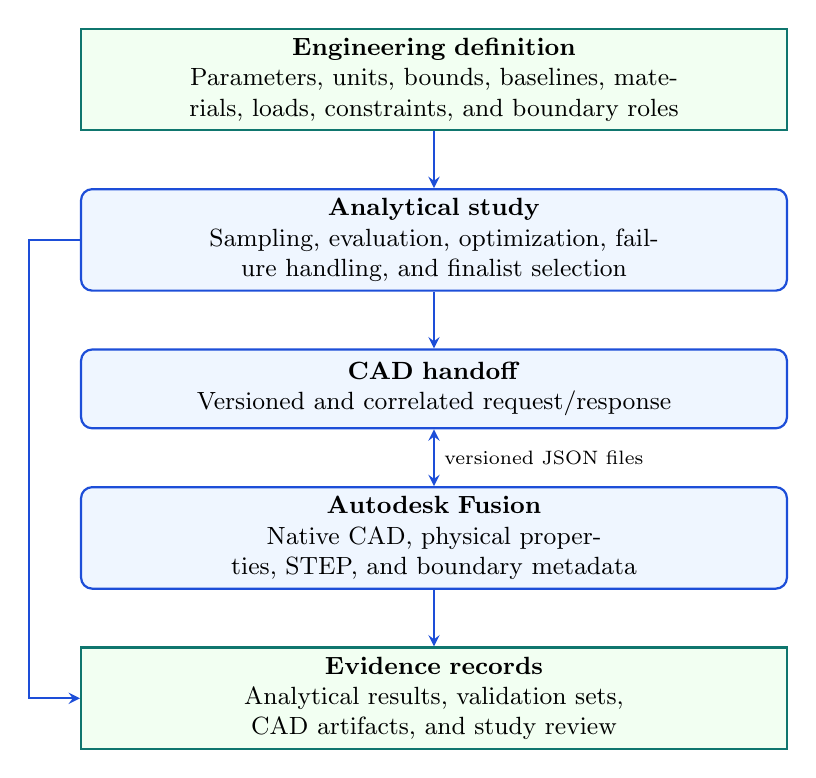
\begin{tikzpicture}[
    node distance=0.72cm,
    box/.style={
        rectangle,
        rounded corners,
        draw=nemoblue,
        fill=nemolight,
        thick,
        text width=0.72\textwidth,
        minimum height=1.0cm,
        align=center,
        font=\small
    },
    data/.style={
        rectangle,
        draw=nemoteal,
        fill=green!5,
        thick,
        text width=0.72\textwidth,
        minimum height=1.0cm,
        align=center,
        font=\small
    }
]
\node[data] (manifest) {\textbf{Engineering definition}\\
Parameters, units, bounds, baselines, materials, loads, constraints, and
boundary roles};
\node[box,below=of manifest] (engine) {\textbf{Analytical study}\\
Sampling, evaluation, optimization, failure handling, and finalist selection};
\node[box,below=of engine] (bridge)
{\textbf{CAD handoff}\\Versioned and correlated request/response};
\node[box,below=of bridge] (fusion)
{\textbf{Autodesk Fusion}\\Native CAD, physical properties, STEP, and
boundary metadata};
\node[data,below=of fusion] (records) {\textbf{Evidence records}\\
Analytical results, validation sets, CAD artifacts, and study review};

\draw[arrow] (manifest) -- (engine);
\draw[arrow] (engine) -- (bridge);
\draw[arrow,<->] (bridge) -- node[right,font=\scriptsize]{versioned JSON files} (fusion);
\draw[arrow] (fusion) -- (records);
\draw[arrow] (engine.west) -- ++(-0.65,0) |- (records.west);
\end{tikzpicture}
\caption{NEMO study workflow and evidence flow}
\label{fig:system-architecture}
\end{figure}

The analytical and CAD stages run in separate Python environments. Their
separation allows the search to use the required scientific dependencies while
Fusion retains its native application environment. A small versioned exchange
passes candidate parameters to Fusion and returns geometry properties and
boundary evidence. Autodesk defines the application lifecycle for Fusion
scripts and add-ins \cite{autodeskAddins}.

\section{Engineering Models}
\label{sec:engineering-models}

\subsection{Common Engineering Definition}
\label{sec:part-definition}

Each component was represented by one engineering definition containing its
design variables, units, lower and upper bounds, baseline dimensions, material
properties, design load, acceptance criteria, fixed geometry, and required
boundary roles. Most dimensions are expressed in millimetres; the stabilizer
spar locations are percentages of local chord. Lengths were converted to
metres for the SI calculations, while stress and displacement were reported in
MPa and millimetres. The same definition governed analytical evaluation,
optimization, candidate selection, and CAD generation so that a change in
load, bound, or unit was not applied differently at successive stages.

\subsection{Bracket}
\label{sec:bracket-definition}

The bracket represents a foundation for a 50~kg auxiliary unit. The design
load uses a project dynamic factor of 3:

\begin{equation}
F_d=mg\gamma_d=50(9.81)(3)=1471.5~\mathrm{N}.
\label{eq:bracket-load}
\end{equation}

The dynamic factor is an engineering envelope. It is not a modal, shock, or
vessel-motion result. The analytical calculation retains 1471.5~N. The current
Fusion input dialog does not accept the decimal force value used in this
workflow. The manual study therefore uses the conservative integer value
1472~N, a difference of approximately 0.034\%.

The project-defined Aluminum 6061-T6 properties are density
2700~kg/m$^3$, yield strength 276~MPa, Young's modulus 68.9~GPa, and
Poisson ratio 0.33. Table~\ref{tab:bracket-parameters} gives the variables.

\begin{table}[H]
\centering
\caption{Bracket design variables}
\label{tab:bracket-parameters}
\begin{tabularx}{\textwidth}{Xcrrr}
\toprule
\textbf{Variable} & \textbf{Unit} & \textbf{Lower} & \textbf{Baseline} &
\textbf{Upper}\\
\midrule
Baseplate length & mm & 100 & 150 & 200\\
Baseplate width & mm & 80 & 100 & 150\\
Baseplate thickness & mm & 4 & 8 & 15\\
Rib height & mm & 20 & 40 & 60\\
Rib thickness & mm & 3 & 6 & 10\\
Fillet radius & mm & 2 & 5 & 10\\
\bottomrule
\end{tabularx}
\end{table}

The fixed geometry includes four 10~mm mounting holes and two ribs. The
screening acceptance criteria are $FOS\geq2.5$ and
$\delta\leq0.5$~mm. These limits are project criteria and do not replace a
governing marine rule set.

\subsubsection{Analytical formulation}
\label{sec:bracket-model}

All geometric dimensions enter the equations in meters. The approximate
volume contains the rectangular baseplate, four-hole subtraction, two
triangular ribs, and a fillet contribution:

\begin{equation}
V_b =
LWt_b
-n_h\pi\left(\frac{d_h}{2}\right)^2t_b
+n_r\frac{Lh_rt_r}{2}
+n_r\frac{\pi r_f^2}{4}\max(0.35W,t_r).
\label{eq:bracket-volume}
\end{equation}

The bracket mass is

\begin{equation}
m_b=\rho V_b.
\label{eq:bracket-mass}
\end{equation}

The equivalent cantilever moment is

\begin{equation}
M_b=F_de,\qquad
e=\max(0.03,0.35L+0.02).
\label{eq:bracket-moment}
\end{equation}

The effective section modulus combines the baseplate and rib terms:

\begin{equation}
Z_{\mathrm{eff}}=
\frac{Wt_b^2}{6}
+0.65n_r\frac{t_rh_r^2}{6}.
\label{eq:bracket-section-modulus}
\end{equation}

The stress estimate includes a fillet-dependent concentration factor:

\begin{align}
K_t&=\max\left(1.08,1.35-\frac{r_f[\mathrm{mm}]}{40}\right),
\label{eq:bracket-kt}\\
\sigma_b&=\frac{M_b}{Z_{\mathrm{eff}}}K_t.
\label{eq:bracket-stress}
\end{align}

The effective second moment of area is

\begin{equation}
I_{\mathrm{eff}}=
\frac{Wt_b^3}{12}
+0.45n_r\frac{t_rh_r^3}{36},
\label{eq:bracket-inertia}
\end{equation}

and the tip-equivalent displacement is

\begin{equation}
\delta_b=\frac{F_de^3}{3EI_{\mathrm{eff}}}.
\label{eq:bracket-displacement}
\end{equation}

The yield-based factor of safety is

\begin{equation}
FOS_b=\frac{\sigma_y}{\sigma_b}.
\label{eq:bracket-fos}
\end{equation}

The equations preserve the expected broad trends. Increased plate or rib
thickness increases mass and stiffness. Increased rib height strongly
increases bending stiffness. Increased fillet radius reduces the assumed
stress concentration. The model does not calculate bolt bearing, bolt
preload, weld-group stress, weld-toe fatigue, local plate bending, contact, or
three-dimensional load sharing.

\subsection{Padeye}
\label{sec:padeye-definition}

The padeye represents a lifting point for a 500~kg working mass with a dynamic
factor of 3:

\begin{equation}
F_d=500(9.81)(3)=14\,715~\mathrm{N}.
\label{eq:padeye-load}
\end{equation}

The project-defined S275 properties are density 7850~kg/m$^3$, yield strength
275~MPa, Young's modulus 210~GPa, and Poisson ratio 0.30. The fixed pin-hole
diameter is 50~mm, and two gussets reinforce the lug. The criteria are
$FOS\geq2.5$ and $\delta\leq0.5$~mm.

\begin{table}[H]
\centering
\caption{Padeye design variables}
\label{tab:padeye-parameters}
\begin{tabularx}{\textwidth}{Xcrrr}
\toprule
\textbf{Variable} & \textbf{Unit} & \textbf{Lower} & \textbf{Baseline} &
\textbf{Upper}\\
\midrule
Base length & mm & 220 & 260 & 320\\
Base width & mm & 150 & 180 & 230\\
Base thickness & mm & 8 & 14 & 22\\
Lug height & mm & 140 & 180 & 230\\
Lug thickness & mm & 12 & 20 & 30\\
Neck width & mm & 80 & 100 & 140\\
Gusset height & mm & 70 & 110 & 120\\
Gusset thickness & mm & 6 & 10 & 18\\
Fillet radius & mm & 8 & 15 & 25\\
\bottomrule
\end{tabularx}
\end{table}

\subsubsection{Analytical formulation}
\label{sec:padeye-model}

The volume model combines the doubler plate, a tapered lug and circular crown,
the 50~mm hole subtraction, two triangular gussets, and a fillet
approximation. This representation follows the native generator closely enough
for a mass consistency check, but it is not an exact boundary-representation
calculation.

The structural model calculates four candidate stresses. The net-section
tension stress uses the remaining ligament at the hole and a
fillet-dependent stress factor. The nominal bearing stress is

\begin{equation}
\sigma_{\mathrm{bearing}}=
\frac{F_d}{d_p t_l},
\label{eq:padeye-bearing}
\end{equation}

where $d_p$ is pin diameter and $t_l$ is lug thickness. The shear-out
estimate uses the two load paths between the hole and the outer edge:

\begin{equation}
\tau_{\mathrm{out}}=
\frac{F_d}{2A_{\mathrm{shear}}}.
\label{eq:padeye-shearout}
\end{equation}

A lateral-bending estimate represents an assumed 25\% side-load component.
The reported padeye stress is

\begin{equation}
\sigma_p=\max\left(
\sigma_{\mathrm{net}},
\sigma_{\mathrm{bearing}},
\sqrt{3}\tau_{\mathrm{out}},
\sigma_{\mathrm{lateral}}
\right).
\label{eq:padeye-governing-stress}
\end{equation}

The displacement combines axial and lateral terms, and the factor of safety is
$FOS_p=\sigma_y/\sigma_p$. This model ranks candidates by several relevant
nominal modes. It does not model a separate pin, pin clearance, nonlinear
contact, local peak stress, weld geometry, or fatigue. These limitations
define the later FEA and design-code work.

\subsection{Stabilizer}
\label{sec:stabilizer-definition}

The stabilizer retains a NACA 0015 outer envelope with 800~mm span, 500~mm root
chord, 250~mm tip chord, 12-degree sweep, and 8~mm trailing edge. It has a
560~mm by 160~mm by 18~mm root flange and three ribs at 25\%, 50\%, and 75\%
span.

The project-defined Aluminum 6061-T6 properties match the bracket. The
prescribed resultant follows

\begin{equation}
F_d=\frac{1}{2}\rho_wV^2SC_L\gamma_d,
\label{eq:stabilizer-load-general}
\end{equation}

where seawater density is 1025~kg/m$^3$, speed is 8~m/s, planform area is
0.3~m$^2$, lift coefficient is 0.8, and the dynamic factor is 1.5. Thus

\begin{equation}
F_d=
\frac{1}{2}(1025)(8^2)(0.3)(0.8)(1.5)
=11\,808~\mathrm{N}.
\label{eq:stabilizer-load}
\end{equation}

Four pressure bands use relative weights 1.00, 0.93, 0.75, and 0.40. These are
declared engineering assumptions, not CFD data. The screening criteria are
$FOS\geq2.5$ and tip displacement no more than 5~mm.

\begin{table}[H]
\centering
\caption{Stabilizer design variables}
\label{tab:stabilizer-parameters}
\begin{tabularx}{\textwidth}{Xcrrr}
\toprule
\textbf{Variable} & \textbf{Unit} & \textbf{Lower} & \textbf{Baseline} &
\textbf{Upper}\\
\midrule
Skin thickness & mm & 4 & 7 & 12\\
Front spar position & \% chord & 25 & 30 & 38\\
Rear spar position & \% chord & 58 & 65 & 72\\
Front spar thickness & mm & 4 & 8 & 14\\
Rear spar thickness & mm & 4 & 6 & 12\\
Rib thickness & mm & 3 & 5 & 9\\
Root insert length & mm & 120 & 180 & 260\\
Root insert thickness & mm & 8 & 12 & 20\\
Root fillet radius & mm & 12 & 25 & 40\\
\bottomrule
\end{tabularx}
\end{table}

\subsubsection{Analytical formulation}
\label{sec:stabilizer-model}

The volume model combines the two-sided skin, front and rear spar webs, three
internal ribs, root insert, fixed flange, and root-fillet approximation. The
NACA thickness equation estimates the local spar height at each chord
position. The root section combines skin, spar, and insert contributions to
the second moment of area.

The root bending moment uses a resultant centroid at 40\% span:

\begin{equation}
M_r=0.40F_db.
\label{eq:stabilizer-moment}
\end{equation}

The model calculates a nominal root bending stress $\sigma_b$ and shear stress
$\tau$. A root-fillet factor $K_t$ modifies the bending term. The equivalent
stress is

\begin{equation}
\sigma_s=
\sqrt{(K_t\sigma_b)^2+3\tau^2}.
\label{eq:stabilizer-stress}
\end{equation}

The tip displacement estimate is

\begin{equation}
\delta_s=\frac{F_db^3}{8EI_{\mathrm{eff}}}.
\label{eq:stabilizer-displacement}
\end{equation}

The model does not derive the pressure field. It also omits torsional
deflection, shell buckling, panel crippling, local skin--spar stress, fatigue,
fluid--structure interaction, and root-bearing detail. It therefore supports
structural screening under a prescribed load, not hydrodynamic optimization.

\section{Design-Space Exploration and Optimization}
\label{sec:search-method}

\subsection{Evaluation and Failure Handling}
\label{sec:evaluation-contract}

Each evaluator returns a structured record with volume, mass, maximum stress,
factor of safety, maximum displacement, objective, status, and error. It first
checks that the part exists, all required parameters are present, values are
finite, values lie within bounds, and the requested evaluation mode is
available.

Invalid inputs and unavailable evaluators return a failed record with
objective $10^9$. The analytical optimizer can continue after such a record.
A CAD-only response has partial status because it can contain valid mass and
artifacts while structural metrics remain unavailable. The reserved
\code{open\_fea} mode deliberately returns a controlled failure. No Gmsh or
CalculiX result is fabricated.

\subsection{Latin-Hypercube Exploration}
\label{sec:sampling-method}

Each part used 60 Latin-hypercube samples with seed 42. The sampler operated in
the scaled unit cube. Each variable was divided into 60 intervals. A random
point was selected within each interval, and independently permuted variable
columns formed the multi-dimensional vectors. The inverse scaling in
Equation~\ref{eq:variable-scaling} produced physical values.

The sampler evaluated all points, retained failed records, and counted
feasible candidates. A feasible candidate met both the factor-of-safety and
displacement constraints. Promising feasible sampled designs supplied two of
the three optimization starts.

\subsection{Bounded Multi-Start Optimization}
\label{sec:optimization-method}

The pure-Python optimizer operated on scaled coordinates. Each part used three
starts:

\begin{enumerate}
    \item the configured baseline;
    \item a promising low-mass feasible sample; and
    \item a second promising feasible sample that provided another basin or
    parameter combination.
\end{enumerate}

Each run permitted at most 80 simplex iterations. The optimizer converted each
trial point to physical units, evaluated the part, cached repeated vectors,
and appended each unique evaluation to the run log. The simplex stopped at the
iteration limit or when the objective spread met the configured tolerance.

\begin{figure}[H]
\centering
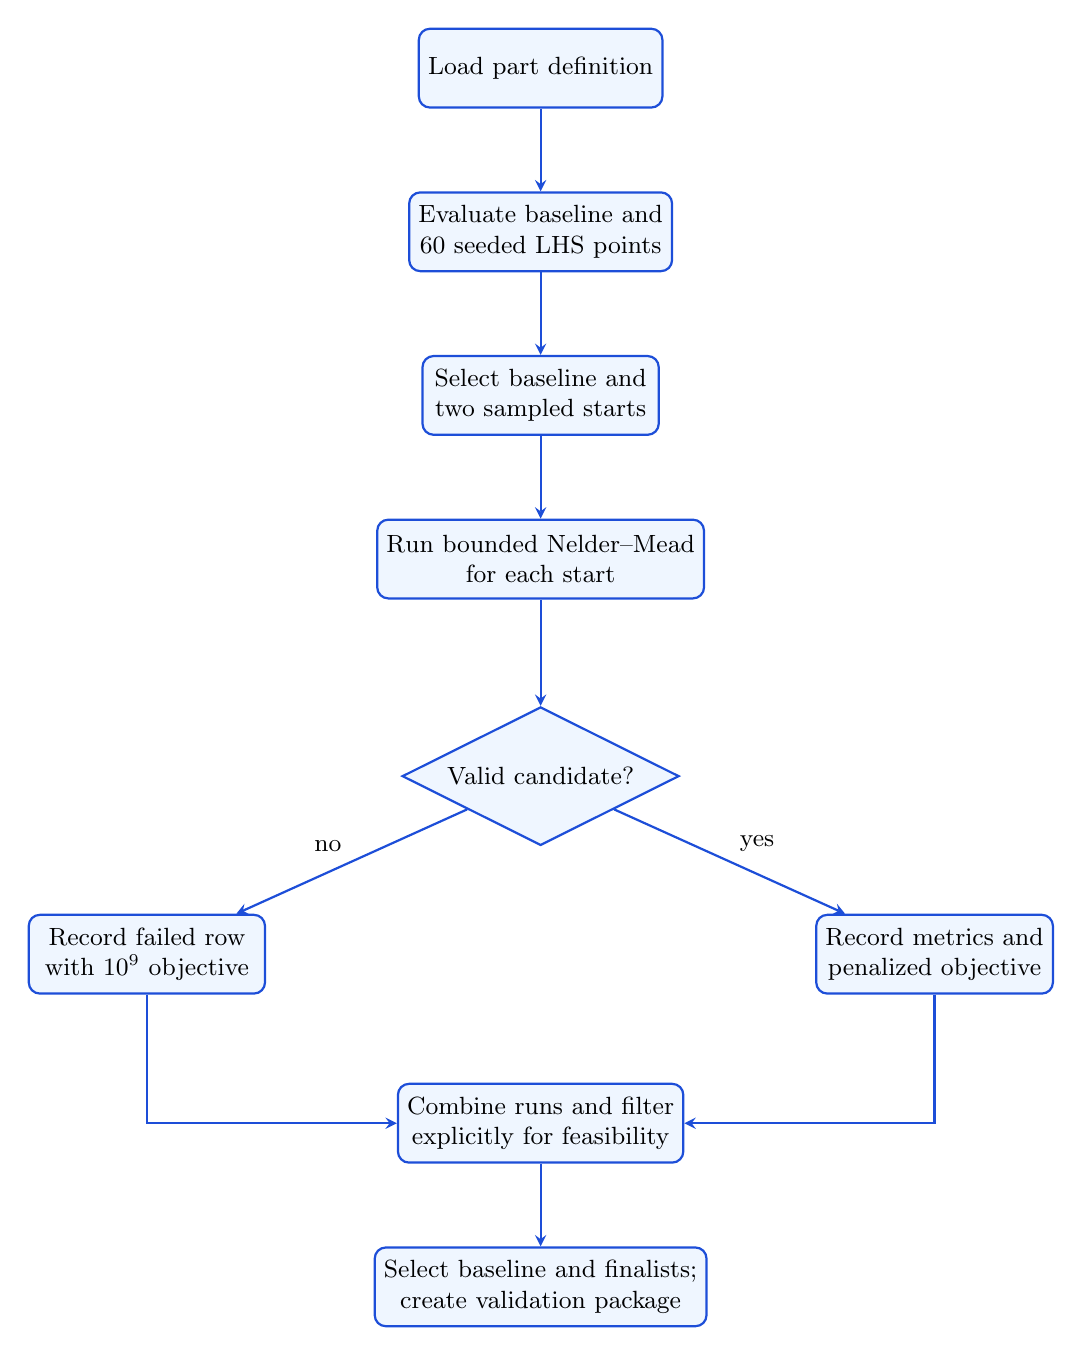
\begin{tikzpicture}[node distance=1.05cm,every node/.style={font=\small}]
\node[startstop] (start) {Load part definition};
\node[process,below=of start] (baseline) {Evaluate baseline and\\60 seeded LHS points};
\node[process,below=of baseline] (starts) {Select baseline and\\two sampled starts};
\node[process,below=of starts] (nm) {Run bounded Nelder--Mead\\for each start};
\node[decision,below=1.35cm of nm] (valid) {Valid candidate?};
\node[process,below left=1.3cm and 2.6cm of valid] (fail) {Record failed row\\with $10^9$ objective};
\node[process,below right=1.3cm and 2.6cm of valid] (metrics) {Record metrics and\\penalized objective};
\node[process,below=3.0cm of valid] (filter) {Combine runs and filter\\explicitly for feasibility};
\node[startstop,below=of filter] (package) {Select baseline and finalists;\\create validation package};

\draw[arrow] (start) -- (baseline);
\draw[arrow] (baseline) -- (starts);
\draw[arrow] (starts) -- (nm);
\draw[arrow] (nm) -- (valid);
\draw[arrow] (valid) -- node[above left]{no} (fail);
\draw[arrow] (valid) -- node[above right]{yes} (metrics);
\draw[arrow] (fail) |- (filter);
\draw[arrow] (metrics) |- (filter);
\draw[arrow] (filter) -- (package);
\end{tikzpicture}
\caption{Sampling, optimization, and finalist-selection procedure}
\label{fig:optimization-flow}
\end{figure}

The selection step is deliberately separate from the optimizer's minimum
objective. The validation package sorts only feasible rows by mass. It retains
five finalists so that the lightest design does not become the only candidate
for later FEA.

\subsection{Results Recording and Review}
\label{sec:logging-method}

Each evaluated candidate was recorded with its part identifier, parameter
values, calculated metrics, feasibility status, objective, and any evaluation
error. Run-level metadata preserved the seed and search context. A dashboard
was used to inspect convergence, parameter activity, mass, constraint use, and
failed evaluations without changing the underlying results.

\section{CAD Generation and Boundary Definition}
\label{sec:cad-method}

\subsection{Versioned CAD Handoff}
\label{sec:fusion-bridge}

Each CAD request identifies the schema, component, run, iteration, evaluation
mode, parameter values, and required artifacts. A legacy form is retained for
the original bracket demonstration. Requests and responses are written
atomically, and each returned result is accepted only when its run and
iteration identifiers match the candidate under evaluation. This prevents a
partial or stale exchange from being interpreted as current evidence.

\begin{figure}[H]
\centering
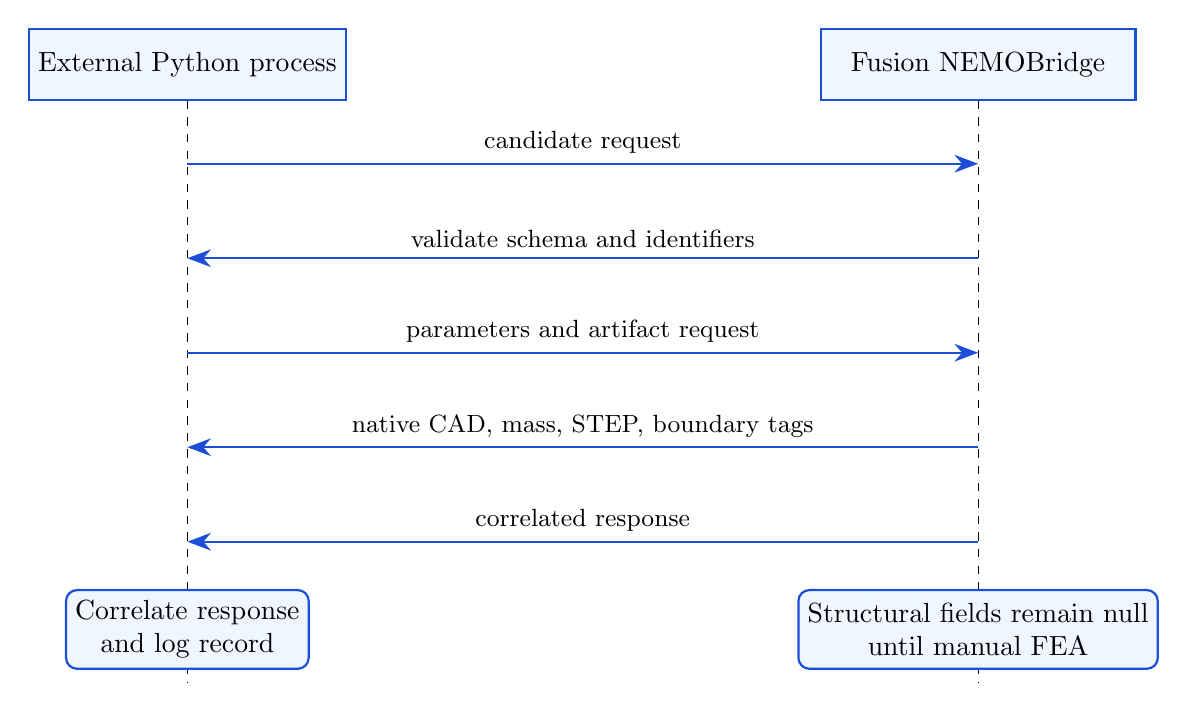
\begin{tikzpicture}[
    node distance=1.4cm and 2.0cm,
    lifeline/.style={rectangle,draw=nemoblue,fill=nemolight,thick,
    minimum width=4.0cm,minimum height=0.9cm,align=center},
    msg/.style={-{Stealth[length=3mm]},thick,draw=nemoblue}
]
\node[lifeline] (external) {External Python process};
\node[lifeline,right=6.0cm of external] (fusion) {Fusion NEMOBridge};
\draw[dashed] (external.south) -- ++(0,-7.4);
\draw[dashed] (fusion.south) -- ++(0,-7.4);
\draw[msg] ($(external.south)+(0,-0.8)$) --
node[above,font=\small]{candidate request} ($(fusion.south)+(0,-0.8)$);
\draw[msg] ($(fusion.south)+(0,-2.0)$) --
node[above,font=\small]{validate schema and identifiers}
($(external.south)+(0,-2.0)$);
\draw[msg] ($(external.south)+(0,-3.2)$) --
node[above,font=\small]{parameters and artifact request}
($(fusion.south)+(0,-3.2)$);
\draw[msg] ($(fusion.south)+(0,-4.4)$) --
node[above,font=\small]{native CAD, mass, STEP, boundary tags}
($(external.south)+(0,-4.4)$);
\draw[msg] ($(fusion.south)+(0,-5.6)$) --
node[above,font=\small]{correlated response}
($(external.south)+(0,-5.6)$);
\node[process,below=6.2cm of external] (log) {Correlate response\\and log record};
\node[process,below=6.2cm of fusion] (partial) {Structural fields remain null\\until manual FEA};
\end{tikzpicture}
\caption{Serialized Fusion request and response sequence}
\label{fig:bridge-sequence}
\end{figure}

The handoff permits one active CAD request at a time. This serialized approach
favours traceability over throughput and prevents two candidates from
competing for the same exchange state.

\subsection{Native CAD Generation}
\label{sec:cad-generation}

The Fusion generator uses the same engineering definitions as the analytical
study while remaining within Fusion's separate Python environment.

\subsubsection{Bracket}

The bracket generator creates a rectangular baseplate, cuts four mounting
holes, creates two triangular ribs, joins the bodies, and applies four long
rib-root fillets. It checks that the result is one connected solid with
positive volume. It identifies the mounting-hole cylindrical faces as the
fixed-support role and the four upper sloping rib faces as the
equipment-load role.

\subsubsection{Padeye}

The padeye generator creates the doubler plate, tapered lug, circular crown,
pin bore, two root fillets, and two overlapping gussets. It requires one
connected solid. The underside of the doubler plate supplies the
fixed-support role. The cylindrical pin-hole region supplies the
pin-bearing role.

\subsubsection{Stabilizer}

The stabilizer generator creates the root flange, lofted NACA outer envelope,
root fillet, hollow interior, front and rear spars, three ribs, root insert,
and pressure-band splits. It requires one connected solid. The root flange
provides the fixed support. Four surface regions provide the pressure bands,
and a tip region provides the displacement monitor.

Autodesk exposes physical-property and export functions through the public API
\cite{autodeskPhysicalProperties,autodeskExport}. \NEMO\ records mass and
volume from the generated component and exports STEP for downstream exchange.
STL is optional because it is a tessellated artifact rather than the preferred
solid exchange format.

\subsection{Semantic Boundary Definition}
\label{sec:boundary-method}

For each required role, the generator stores one or more face signatures.
Available fields include area, centroid, normal, bounding box, and cylindrical
geometry. The generator fails the sweep acceptance check if a required role
has no matching face.

This metadata has three functions. First, it documents what the generator
believed the load or support region to be. Second, it helps the engineer find
the same region in the manual study. Third, it makes topology problems visible
during a sweep.

It does not automatically apply the FEA boundary condition. The engineer must
still display the faces, compare them with the intended load path, and reject
an incorrect selection.

\section{Verification and Validation}
\label{sec:verification-validation-method}

\subsection{CAD Generator Verification}
\label{sec:cad-sweep-method}

Each generator was tested with its configured baseline and 20 seeded
Latin-hypercube vectors. The acceptance criteria for each of the 21 cases were:

\begin{enumerate}
    \item the request completed without an uncontrolled exception;
    \item the result contained exactly one connected solid;
    \item the physical volume was positive;
    \item STEP export completed;
    \item boundary metadata export completed; and
    \item every required semantic boundary role matched at least one face.
\end{enumerate}

The sweep does not solve FEA. It tests whether the generator and boundary
contract remain usable across the bounded design space. It is intentionally
separate from the offline test suite because it requires an open Fusion
session and mutates the shared live channel.

\subsection{Finalist Validation Preparation}
\label{sec:validation-package-method}

For each component, the baseline and five light feasible candidates were
assembled into a validation set. Each record retained its parameters,
analytical predictions, intended material and boundaries, CAD status and mass,
and fields for later FEA inputs, outputs, convergence evidence, and engineering
disposition. This preserved the connection between a solver image and the
candidate to which it belonged.

\subsection{Bracket Static Stress Studies}
\label{sec:bracket-poc-method}

The bracket proof of concept continued from the analytical finalist set into
Fusion Static Stress. Aluminum 6061 was assigned to the generated bracket, the
four mounting-hole surfaces represented the initial fixed-support
idealization, and the four upper sloping rib faces represented the equipment
load interface. The intended total downward load was 1472~N, obtained by
rounding the analytical design load of 1471.5~N to the integer input used for
the study.

Two exploratory studies were reviewed. Their material assignment, boundary
regions, mesh information, result magnitudes, and result locations were
compared with the engineering definition. The review also checked whether the
applied force was a total load rather than a load repeated on every selected
face. The images and findings from both studies are presented and interpreted
in Section~\ref{sec:bracket-fea-result}.

\subsection{Static Stress Assessment Criteria}
\label{sec:fea-quality-procedure}

Study credibility was assessed from the material properties, applied-load
magnitude and direction, support and contact idealizations, mesh order and
refinement, reaction balance, result locations, and stability under mesh
change. Maximum von Mises stress, minimum factor of safety, and maximum
displacement were considered only after these input and numerical checks.
Peaks at constrained edges were treated cautiously because they can represent
local singular behaviour. Even an acceptable linear-static study would cover
only the stated load case and would not establish fatigue, buckling, weld,
bolt, corrosion, impact, or classification compliance.

\subsection{Extension to Padeye FEA}
\label{sec:padeye-fea-method}

The padeye study will follow the same evidence sequence with part-specific
boundaries and result regions. The underside of the doubler plate will provide
the first fixed-support idealization. The 14\,715~N design load will act
through the pin-bearing region.

An initial linear screening model can use a distributed bearing load on the
hole surface. A later detailed model should include a separate pin, clearance,
contact, and any required nonlinear behavior. The review regions are the
loaded hole, crown, net section, shear-out ligaments, lug root, gusset roots,
doubler interface, and weld lines. Reaction balance must close to
14\,715~N in the applied direction.

The final design assessment must also check the selected lifting code, load
angle range, dynamic factors, material certification, weld class, fabrication
tolerance, inspection, proof load, fatigue, and supporting structure.

\subsection{Extension to Stabilizer FEA}
\label{sec:stabilizer-fea-method}

The stabilizer study will fix the root-flange interface. The 11\,808~N
resultant will be distributed over four pressure bands. The band forces are
calculated by normalizing the weights 1.00, 0.93, 0.75, and 0.40. Pressure on
each band equals its force divided by its actual CAD face area.

The study will monitor tip displacement and inspect the root fillet, front and
rear spars, skin--spar intersections, rib junctions, insert termination, root
flange, and trailing edge. Shell or solid element choice must represent the
thin skins and local joints adequately. Buckling and fatigue require separate
studies.

The prescribed load distribution is an interim structural envelope. A later
hydrodynamic stage must define operational conditions and derive pressure from
an accepted method. The structural model should then include positive and
negative load cases, torsion, actuator loads, and relevant vessel motions.

\subsection{Reproducibility and Method Limitations}
\label{sec:method-verification}

Software verification covered engineering-definition loading, bounds,
baseline feasibility, qualitative model sensitivity, sampling, optimizer
behaviour, controlled failures, results recording, CAD handoff, and finalist
preparation. Fusion sweeps were conducted separately because they depend on an
active desktop application; they checked geometry and boundary evidence but
did not solve FEA.

Exact finalist parameters, analytical results, CAD masses, and solver-study
evidence were retained so that the tables and figures in this report could be
traced to the corresponding candidate. The method improves reproducibility,
but it does not remove uncertainty in the analytical assumptions, candidate
selection, CAD boundary identification, or manual solver setup.

\screeningwarning

The method was designed to reduce candidate count and improve traceability. It
was not designed to certify marine hardware. A future engineering decision
must use verified loads, applicable codes, detailed FEA, uncertainty
assessment, fatigue and fabrication checks, physical testing where required,
and qualified approval.

\chapter{Results and Discussion}
\label{chap:results}

This chapter reports software verification, analytical baselines,
Latin-hypercube exploration, multi-start optimization, finalist selection,
native CAD sweeps, CAD mass checks, and the bracket FEA quality-control
finding. Analytical, CAD, and FEA results are reported separately. The chapter
then answers the research questions and discusses the limitations of the
evidence.

\section{Verification Results}
\label{sec:software-results}

The offline verification campaign passed 27 tests; three Fusion-dependent
tests were excluded from that campaign because they require an active desktop
session. The completed checks covered the engineering definitions and bounds,
baseline feasibility, expected analytical trends, repeatable sampling,
bounded optimization, failed-evaluation containment, results recording, CAD
handoff, candidate preparation, and results review. Native-CAD sweeps were
evaluated separately in Section~\ref{sec:cad-sweep-results}; they did not
perform FEA.

\section{Analytical Optimization Results}
\label{sec:analytical-results}

\subsection{Baselines}
\label{sec:baseline-results}

\screeningwarning

Table~\ref{tab:baseline-results} gives the configured baselines. All three
passed the implemented factor-of-safety and displacement criteria.

\begin{table}[H]
\centering
\caption{Analytical baseline screening results}
\label{tab:baseline-results}
\resizebox{\textwidth}{!}{%
\begin{tabular}{lrrrrr}
\toprule
\textbf{Part} & \textbf{Mass (kg)} & \textbf{Stress (MPa)} &
\textbf{FOS} & \textbf{Deflection (mm)} & \textbf{Volume (m$^3$)}\\
\midrule
Bracket & 0.418125 & 41.5321 & 6.6455 & 0.195642 & 0.000154861\\
Padeye & 8.847625 & 46.1070 & 5.9644 & 0.013429 & 0.001127086\\
Stabilizer & 19.655593 & 86.9853 & 3.1730 & 3.336750 & 0.007279849\\
\bottomrule
\end{tabular}%
}
\end{table}

The bracket and padeye baselines had large yield-based margins. Their
deflection estimates were also well below the project limits. The stabilizer
had less factor-of-safety and displacement margin, although it remained
analytically feasible. These differences affected the available mass
reduction. A highly conservative baseline provides more room for a mass-only
optimizer than a baseline already close to an active constraint.

\subsection{Latin-Hypercube Exploration}
\label{sec:lhs-results}

Each part used 60 samples with seed 42. Table~\ref{tab:lhs-results} summarizes
the feasible counts and lightest feasible sampled designs.

\begin{table}[H]
\centering
\caption{Seeded Latin-hypercube results}
\label{tab:lhs-results}
\begin{tabularx}{\textwidth}{Xrrrr}
\toprule
\textbf{Part} & \textbf{Feasible samples} &
\textbf{Lightest mass (kg)} & \textbf{FOS} &
\textbf{Deflection (mm)}\\
\midrule
Bracket & 55 of 60 & 0.245687 & 10.4945 & 0.073331\\
Padeye & 60 of 60 & 5.923561 & 4.9324 & 0.010449\\
Stabilizer & 47 of 60 & 16.482802 & 2.7674 & 4.107580\\
\bottomrule
\end{tabularx}
\end{table}

The sample stage achieved its three intended purposes. It exercised broad
combinations of bounded variables, identified feasible low-mass starting
points, and showed that the parts had different constraint activity.

The bracket had five infeasible sampled designs, but its lightest feasible
sample still had high factor-of-safety margin. This indicates that broad
random combinations did not automatically exploit the dimensions that control
the screening stress.

All padeye samples were feasible. The result indicates that the declared
bounds and simplified stress model produce a generous feasible region under
the single project load case. It does not prove that every bounded padeye
would pass pin contact, weld, fatigue, or governing lifting rules.

The stabilizer had 13 infeasible samples. Its lightest feasible sample was
already close to both constraints compared with the other parts. The
stabilizer therefore presented the clearest constrained search.

\subsection{Multi-Start Optimization}
\label{sec:multistart-results}

Table~\ref{tab:multistart-results} gives the lightest feasible row found in
each local run. The start names identify the configured baseline and two
sample-derived starts.

\begin{table}[H]
\centering
\caption{Lightest feasible result from each Nelder--Mead start}
\label{tab:multistart-results}
\resizebox{\textwidth}{!}{%
\begin{tabular}{llrrrr}
\toprule
\textbf{Part} & \textbf{Start} & \textbf{Evaluations} &
\textbf{Mass (kg)} & \textbf{FOS} & \textbf{Deflection (mm)}\\
\midrule
\multirow{3}{*}{Bracket}
& Baseline & 132 & 0.126545 & 2.5530 & 0.475840\\
& Sample 1 & 126 & 0.116928 & 2.5208 & 0.396650\\
& Sample 2 & 129 & 0.113396 & 2.5386 & 0.369832\\
\midrule
\multirow{3}{*}{Padeye}
& Baseline & 108 & 3.837083 & 2.8528 & 0.026150\\
& Sample 1 & 116 & 3.609310 & 2.5767 & 0.026789\\
& Sample 2 & 109 & 3.547772 & 2.6224 & 0.027933\\
\midrule
\multirow{3}{*}{Stabilizer}
& Baseline & 110 & 14.414066 & 2.5041 & 3.932243\\
& Sample 1 & 116 & 14.315361 & 2.5149 & 3.822300\\
& Sample 2 & 111 & 14.391670 & 2.5331 & 3.847508\\
\bottomrule
\end{tabular}%
}
\end{table}

Every part benefited from more than one start. The lightest bracket and
padeye feasible designs came from the second sampled start. The lightest
stabilizer feasible design came from the first sampled start. If the study had
used only the configured baseline, the selected masses would have been higher
for all three parts.

The bracket baseline-start result approached the 0.5~mm displacement limit,
while the other two bracket results were governed more clearly by the
factor-of-safety limit. The padeye displacement remained far from 0.5~mm in
all runs, so its yield-based stress controlled the search. The stabilizer
operated close to the factor-of-safety limit while using approximately
76--79\% of the permitted displacement.

\subsection{Selected Finalists}
\label{sec:selected-finalists}

The validation packages selected the lightest explicitly feasible candidates.
Table~\ref{tab:selected-finalists} compares the selected finalist with its
baseline.

\begin{table}[H]
\centering
\caption{Selected analytical finalist compared with baseline}
\label{tab:selected-finalists}
\footnotesize
\begin{tabular*}{\textwidth}{@{\extracolsep{\fill}}lrrrrr}
\toprule
\textbf{Part} & \textbf{Baseline (kg)} &
\textbf{Finalist (kg)} & \textbf{Reduction} &
\textbf{Final FOS} & \textbf{Defl. (mm)}\\
\midrule
Bracket & 0.418125 & 0.113396 & 72.9\% & 2.5386 & 0.369832\\
Padeye & 8.847625 & 3.547772 & 59.9\% & 2.6224 & 0.027933\\
Stabilizer & 19.655593 & 14.315361 & 27.2\% & 2.5149 & 3.822300\\
\bottomrule
\end{tabular*}
\end{table}

\begin{figure}[H]
\centering
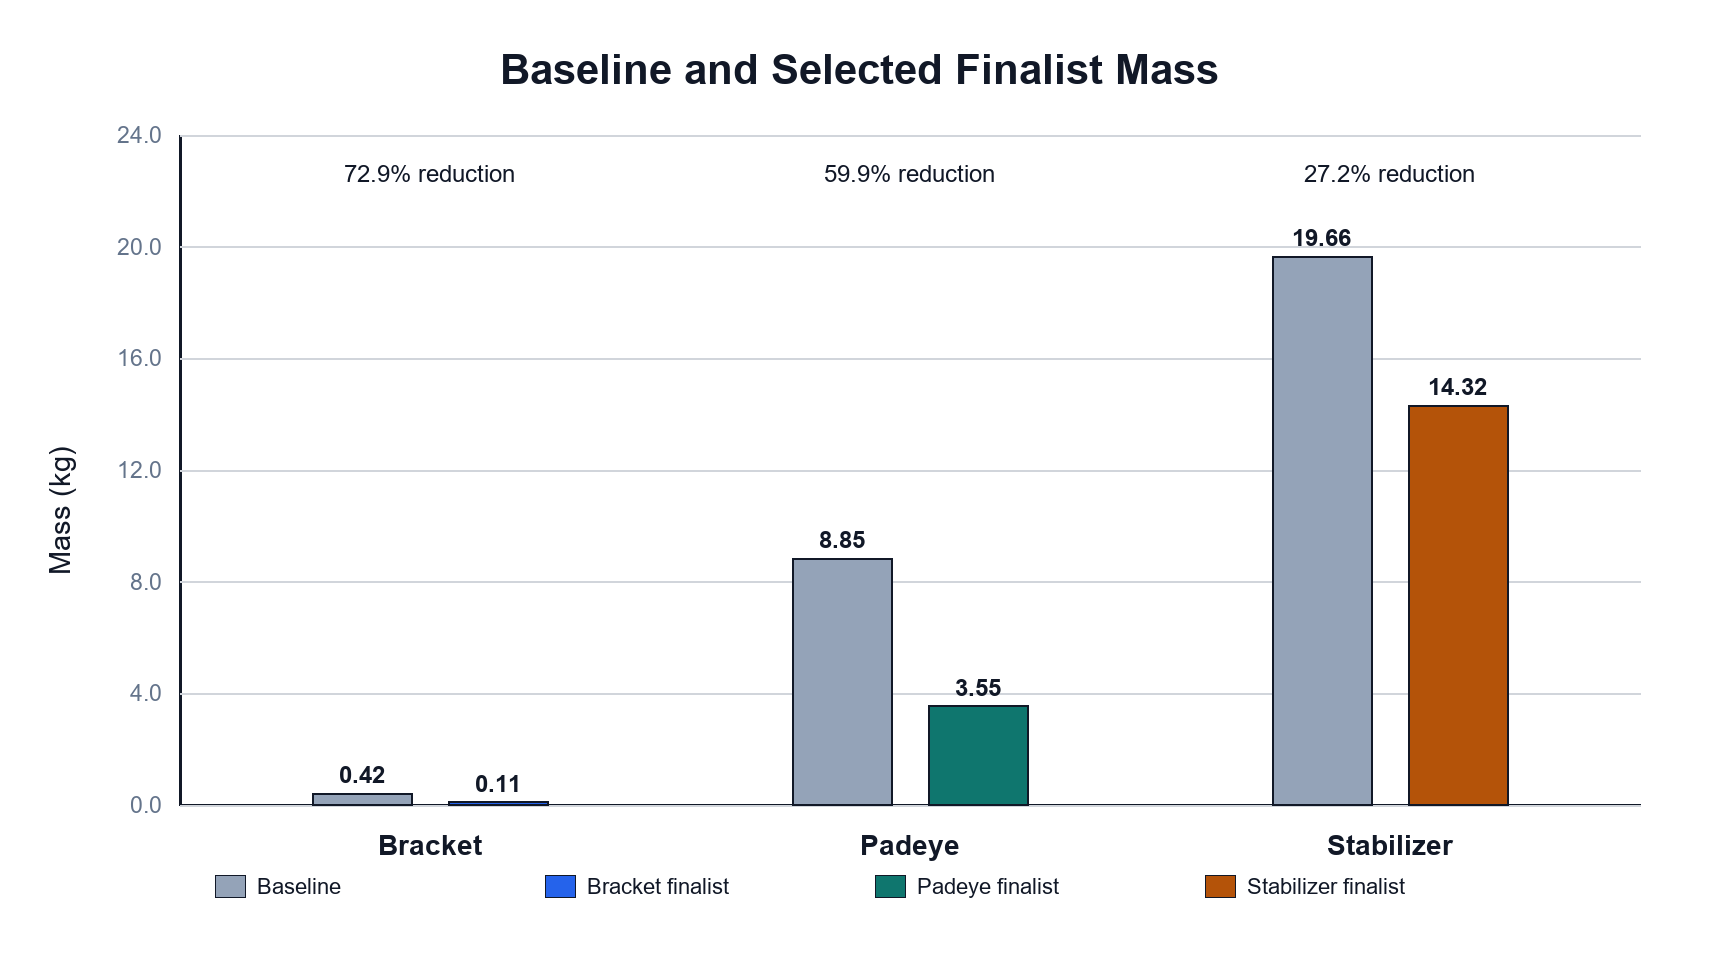
\includegraphics[width=\textwidth]{./images/charts/mass_baseline_finalist.png}
\caption{Analytical baseline and selected-finalist mass. Percentages are
screening reductions within the declared parameterized searches.}
\label{fig:mass-comparison}
\end{figure}

The reductions are large, particularly for the bracket and padeye. They must
be interpreted with the baseline and model scope. The baselines were
configured reference designs, not independently weight-optimized industrial
designs. The equations omit several failure modes. The percentage reduction
therefore measures the opportunity found by the implemented screening model,
not a validated service weight saving.

\subsection{Finalist Constraint Use}
\label{sec:constraint-use}

Figure~\ref{fig:constraint-use} normalizes the finalist responses. A
factor-of-safety ratio of 1.0 means the finalist is exactly at the minimum
factor of safety. A displacement ratio of 1.0 means it is exactly at the
displacement limit.

\begin{figure}[H]
\centering
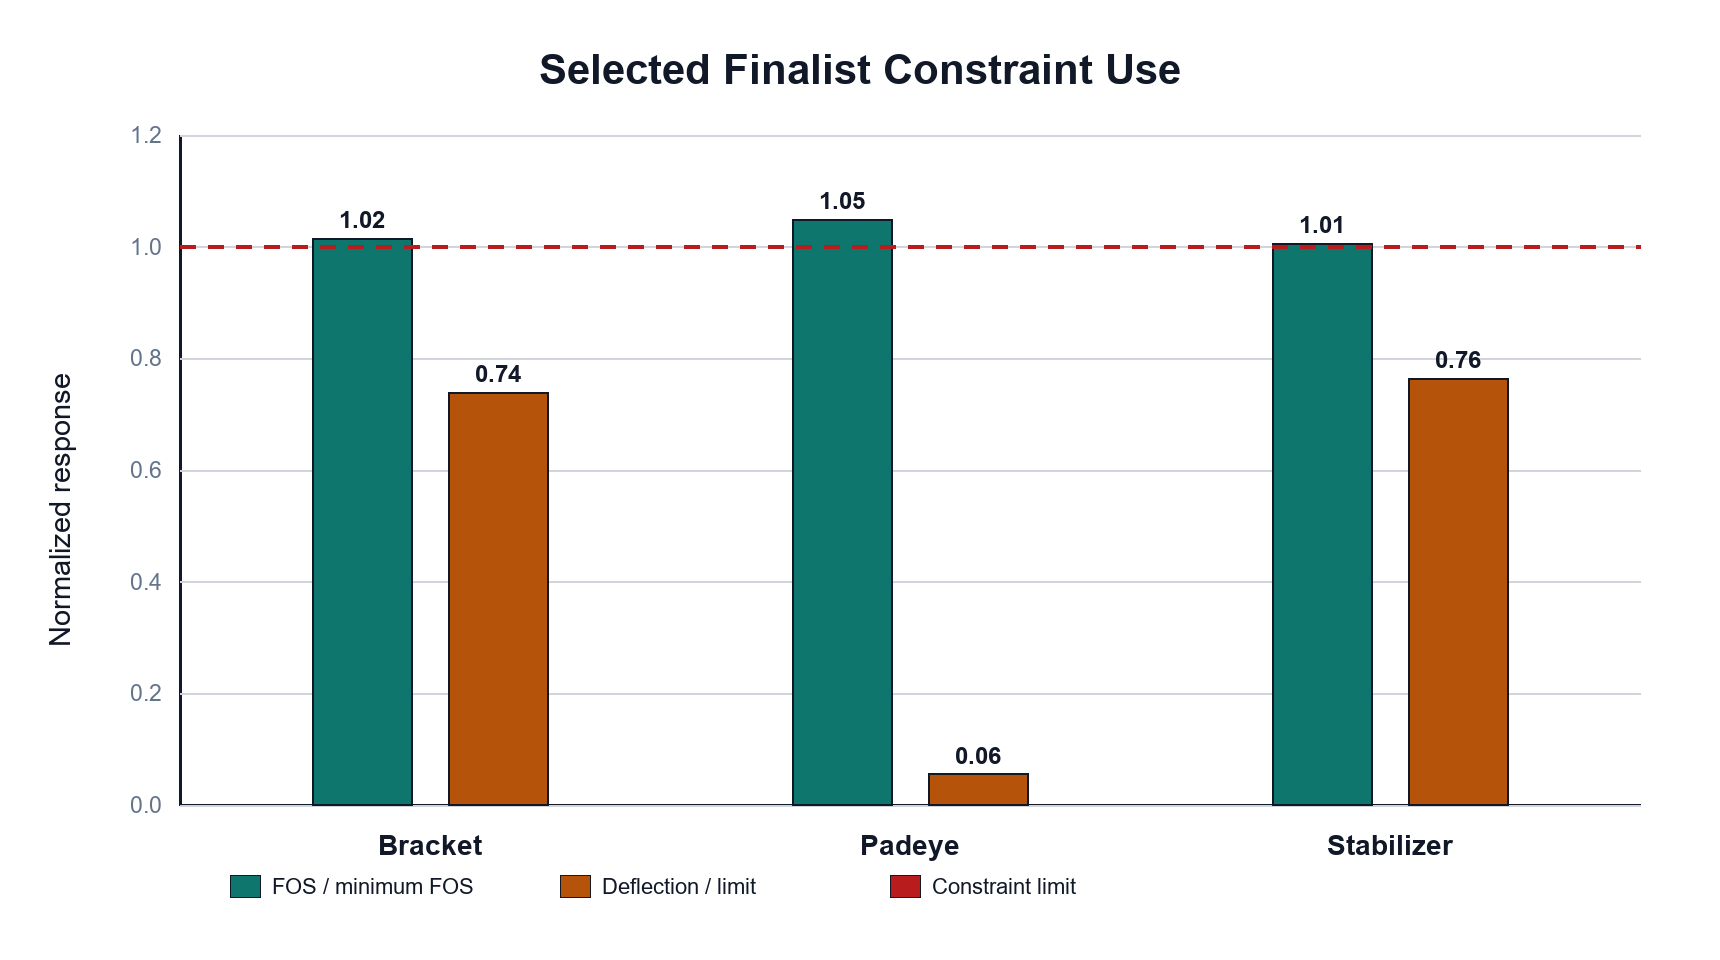
\includegraphics[width=\textwidth]{./images/charts/constraint_use.png}
\caption{Normalized constraint use for the selected analytical finalists}
\label{fig:constraint-use}
\end{figure}

All three finalists have factor-of-safety ratios only slightly above 1.0. This
result is expected from a mass-only search with a yield constraint: the
optimizer removes material until a constraint becomes active. The result also
shows why screening finalists need conservative backup candidates. A small
change in load, material, stress concentration, or model bias could make the
lightest row infeasible.

The bracket displacement ratio is approximately 0.74. The padeye displacement
ratio is approximately 0.056, so the simplified padeye search is almost
entirely controlled by stress. The stabilizer displacement ratio is
approximately 0.76. A later FEA model can change which constraint governs.

\subsection{Parameter Activity}
\label{sec:parameter-activity}

\subsubsection{Bracket}

The selected bracket used approximately 100.03~mm baseplate length,
80.94~mm width, 4.04~mm baseplate thickness, 33.26~mm rib height,
3.00~mm rib thickness, and 3.53~mm fillet radius. The length, width, plate
thickness, and rib thickness were near their lower bounds.

The pattern reflects the analytical equations. Plan dimensions and thickness
reduce volume directly. Rib height retains section depth and bending
resistance with less mass than a uniformly thick plate. This is a plausible
broad trend, but the candidate has little allowance for corrosion,
fabrication tolerance, weld size, bearing, or local plate action. The
lower-bound activity is therefore a prompt to review the bounds and omitted
constraints, not proof that the minimum gauge is suitable.

\subsubsection{Padeye}

The selected padeye used approximately 220.39~mm base length,
150.47~mm base width, 8.05~mm base thickness, 141.73~mm lug height,
12.16~mm lug thickness, 80.00~mm neck width, 70.00~mm gusset height,
6.21~mm gusset thickness, and 25.00~mm fillet radius.

Many thickness and envelope variables approached their lower bounds, while
the fillet radius reached its upper bound. In the analytical model, a large
fillet reduces the assumed concentration factor with a relatively modest
volume cost. The optimizer therefore spends material on the fillet while
reducing other dimensions. A three-dimensional contact and weld model may
change this balance.

\subsubsection{Stabilizer}

The selected stabilizer used approximately 4.01~mm skin, 25.0\% front-spar
position, 72.0\% rear-spar position, 7.85~mm front spar, 6.53~mm rear spar,
5.70~mm ribs, 221.48~mm root insert, 13.66~mm insert thickness, and
18.33~mm root fillet.

The skin approached its lower bound, while the spars moved apart. A larger spar
separation can increase effective section depth. The optimizer retained root
reinforcement to protect the factor-of-safety limit. This response is
consistent with the root-section model. It remains sensitive to the assumed
pressure distribution and omitted torsion and buckling.

\subsection{Penalty Objective and Explicit Feasibility}
\label{sec:penalty-results}

The smallest penalized objective in each stabilizer run was infeasible:

\begin{table}[H]
\centering
\caption{Infeasible minimum-objective rows from the stabilizer searches}
\label{tab:stabilizer-infeasible-objective}
\begin{tabularx}{\textwidth}{Xrrr}
\toprule
\textbf{Start} & \textbf{Objective} & \textbf{Mass (kg)} & \textbf{FOS}\\
\midrule
Baseline & 13.9702 & 13.74695 & 2.38188\\
Sample 1 & 13.7477 & 13.61934 & 2.41042\\
Sample 2 & 13.7335 & 13.61934 & 2.41554\\
\bottomrule
\end{tabularx}
\end{table}

The penalty increased the objective, but the low mass remained attractive
enough to produce a smaller value than the feasible rows. If the package had
selected the minimum objective without a feasibility filter, it would have
promoted a failed design. The implemented selection avoided this error.

This result shows a limitation and a strength. The fixed penalty weight is not
strong enough to make every run's objective minimum feasible. However, the
system does not treat the penalty as the acceptance rule. Explicit feasibility
is the acceptance rule. Future work can compare adaptive penalties,
feasibility-first ranking, or a constrained derivative-free method.

\section{CAD Verification Results}
\label{sec:cad-results}

\subsection{Native CAD Generator Sweeps}
\label{sec:cad-sweep-results}

The final sweeps used generator version 2.4. Table~\ref{tab:cad-sweep-results}
reports their status.

\begin{table}[H]
\centering
\caption{Baseline plus 20-vector native CAD sweep results}
\label{tab:cad-sweep-results}
\begin{tabularx}{\textwidth}{
    >{\raggedright\arraybackslash}X
    rr
    >{\raggedright\arraybackslash}X}
\toprule
\textbf{Part} & \textbf{Artifacts created} & \textbf{Integration passes} &
\textbf{Recorded observation}\\
\midrule
Bracket & 21 of 21 & 21 of 21 &
Completed in approximately 238.19~s.\\
Padeye & 21 of 21 & 21 of 21 &
Completed in approximately 157.19~s.\\
Stabilizer & 21 of 21 & Final read timed out &
All 21 artifacts were created. The outer test reached its 30-minute timeout
while reading the final response; direct artifact audit confirmed generation.\\
\bottomrule
\end{tabularx}
\end{table}

Every audited case contained one connected solid, positive volume, STEP
output, boundary metadata, and non-empty required boundary roles. The result
supports generator behavior over the seeded bounded vectors. It does not prove
behavior for every possible point in the continuous design space.

The stabilizer timeout is reported rather than hidden. The evidence supports
successful artifact generation for all 21 vectors, but it does not support a
claim that the complete outer integration test exited normally. The event
also shows why long-running desktop automation should preserve intermediate
artifacts and per-case records.

\subsection{Analytical and Native-CAD Mass Comparison}
\label{sec:cad-mass-results}

Table~\ref{tab:cad-mass-comparison} compares analytical and Fusion CAD mass
for each baseline and selected finalist. The percentage difference is
calculated relative to the analytical mass.

\begin{table}[H]
\centering
\caption{Analytical and native-CAD mass comparison}
\label{tab:cad-mass-comparison}
\begin{tabularx}{\textwidth}{XXrrr}
\toprule
\textbf{Part} & \textbf{Design} & \textbf{Analytical (kg)} &
\textbf{Fusion CAD (kg)} & \textbf{Difference}\\
\midrule
Bracket & Baseline & 0.418125 & 0.422813 & +1.12\%\\
Bracket & Finalist & 0.113396 & 0.114705 & +1.15\%\\
Padeye & Baseline & 8.847625 & 8.897275 & +0.56\%\\
Padeye & Finalist & 3.547772 & 3.682599 & +3.80\%\\
Stabilizer & Baseline & 19.655593 & 19.297290 & -1.82\%\\
Stabilizer & Finalist & 14.315361 & 14.400328 & +0.59\%\\
\bottomrule
\end{tabularx}
\end{table}

\begin{figure}[H]
\centering
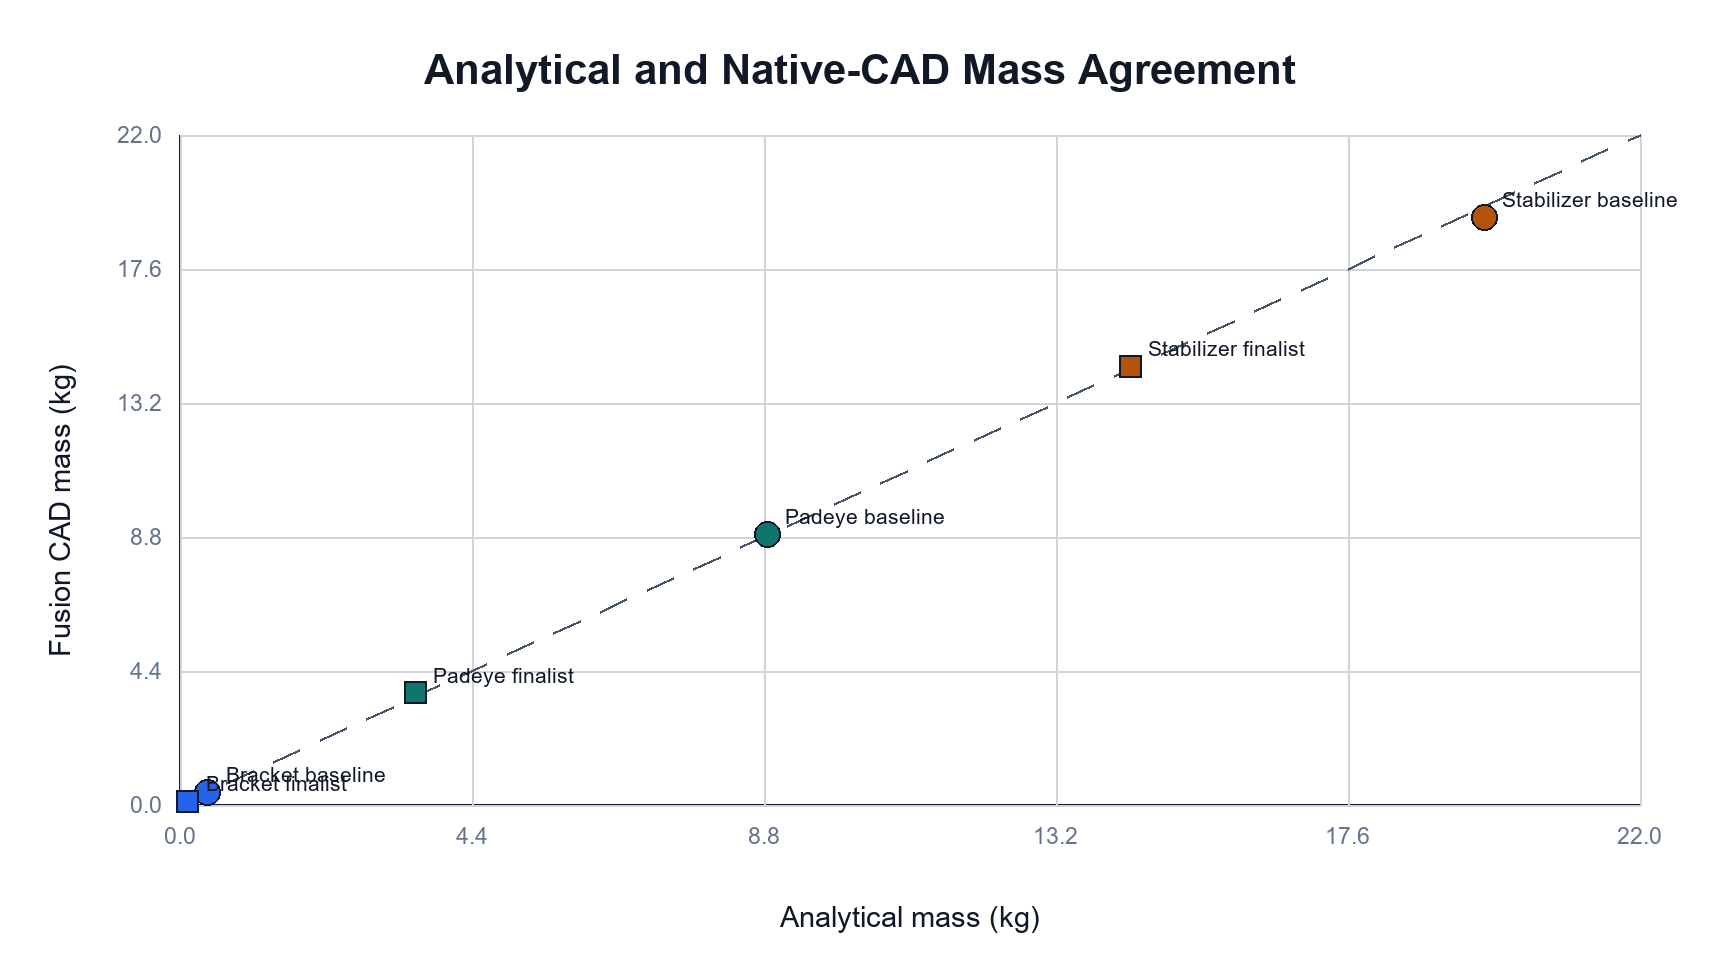
\includegraphics[width=0.86\textwidth]{./images/charts/cad_mass_agreement.png}
\caption{Analytical mass compared with Fusion native-CAD mass. The diagonal
shows exact agreement.}
\label{fig:cad-mass-agreement}
\end{figure}

All six differences were within 3.8\%. The agreement supports the broad
volume approximations used for mass ranking. The padeye finalist showed the
largest difference, which is consistent with greater geometric complexity
around the lug crown, fillets, and gusset intersections.

The agreement does not validate stress. Mass depends primarily on volume and
density. Structural response depends on the load path, section properties,
local geometry, support idealization, contact, and mesh. The CAD response
therefore remains correctly marked as partial.

\section{Bracket Static Stress Study Evidence}
\label{sec:bracket-fea-result}

Two bracket Static Stress reports were available for review. Study~1 records
the first exploratory solve, while Study~2 documents a revised setup with
explicit images of the constrained and loaded faces. Both studies use the
same bracket form and Aluminum 6061 material. Figure~\ref{fig:bracket-study-setups}
shows the progression from the generated geometry to the more clearly
documented boundary conditions.

\begin{figure}[H]
\centering
\begin{minipage}[t]{0.58\textwidth}
\centering
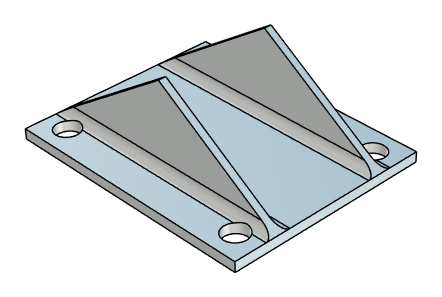
\includegraphics[width=\textwidth]{./images/fusion/study_1_02.png}
\caption*{(a) Study~1 bracket geometry}
\end{minipage}

\vspace{0.3cm}
\begin{minipage}[t]{0.48\textwidth}
\centering
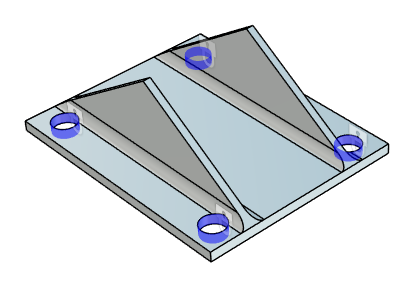
\includegraphics[width=\textwidth]{./images/fusion/study_2_03.png}
\caption*{(b) Study~2 mounting-hole constraints}
\end{minipage}
\hfill
\begin{minipage}[t]{0.48\textwidth}
\centering
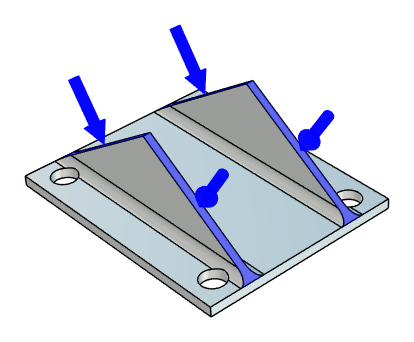
\includegraphics[width=\textwidth]{./images/fusion/study_2_04.png}
\caption*{(c) Study~2 rib-face loading}
\end{minipage}
\caption{Bracket geometry and boundary-condition evidence from the two Fusion
studies. Study~2 makes the four constrained mounting holes and four loaded
upper rib faces visible.}
\label{fig:bracket-study-setups}
\end{figure}

The support regions in Figure~\ref{fig:bracket-study-setups}(b) correspond to
the four cylindrical mounting-hole faces. This is a useful first
idealization of a rigid bolt-down, although it does not represent bolt
preload, clearance, bearing, or contact with the supporting structure. The
arrows in Figure~\ref{fig:bracket-study-setups}(c) confirm that the upper
sloping faces of both ribs were selected for loading. The Study~2 data,
however, record a total magnitude of 1.472~N with \emph{force per entity}
disabled. The intended total was 1472~N. The recorded force also contains both
$X$ and $Z$ components, which makes direction another item that must be
confirmed in the corrected study.

Table~\ref{tab:bracket-study-comparison} summarizes the numerical evidence.
Study~1 does not provide a complete applied-load record, but its reported
1.298~N support reaction and very small response show that it also operated at
a newton-scale load. Study~2 improves traceability but preserves the
factor-of-one-thousand magnitude error.

\begin{table}[H]
\centering
\caption{Comparison of the two exploratory bracket studies}
\label{tab:bracket-study-comparison}
\begin{tabularx}{\textwidth}{
    >{\raggedright\arraybackslash}p{0.25\textwidth}
    >{\raggedright\arraybackslash}X
    >{\raggedright\arraybackslash}X}
\toprule
\textbf{Recorded item} & \textbf{Study 1} & \textbf{Study 2}\\
\midrule
Load evidence &
No complete applied-load table; reported support reaction magnitude
1.298~N &
1.472~N total; force per entity disabled; $X=-0.815$~N and
$Z=-1.226$~N\\
\addlinespace[0.35em]
Mesh evidence &
Parabolic elements; 10\% average element size; no refinement step &
Parabolic elements; 4781 nodes and 2355 elements; 10\% average element
size; no refinement step\\
\addlinespace[0.35em]
Maximum von Mises stress &
0.016~MPa &
0.026~MPa\\
\addlinespace[0.35em]
Minimum factor of safety &
17\,628 &
10\,479\\
\addlinespace[0.35em]
Maximum displacement &
$4.595\times10^{-6}$~mm &
$9.223\times10^{-6}$~mm\\
\addlinespace[0.35em]
Engineering status &
Rejected because the loading is incomplete and inconsistent with the
1.4715~kN design envelope &
Rejected because 1.472~N was applied instead of 1472~N; direction and
reaction balance also require confirmation\\
\bottomrule
\end{tabularx}
\end{table}

The factor-of-safety plots in Figure~\ref{fig:bracket-fos-comparison} are
almost uniformly blue because the display is capped at 8 while the reported
minimum factors of safety exceed ten thousand. The images are therefore
evidence of an unrealistically lightly loaded model, not evidence of a highly
efficient bracket. They also illustrate why a colour plot must be read
together with its legend and input table.

\begin{figure}[H]
\centering
\begin{minipage}{0.88\textwidth}
\centering
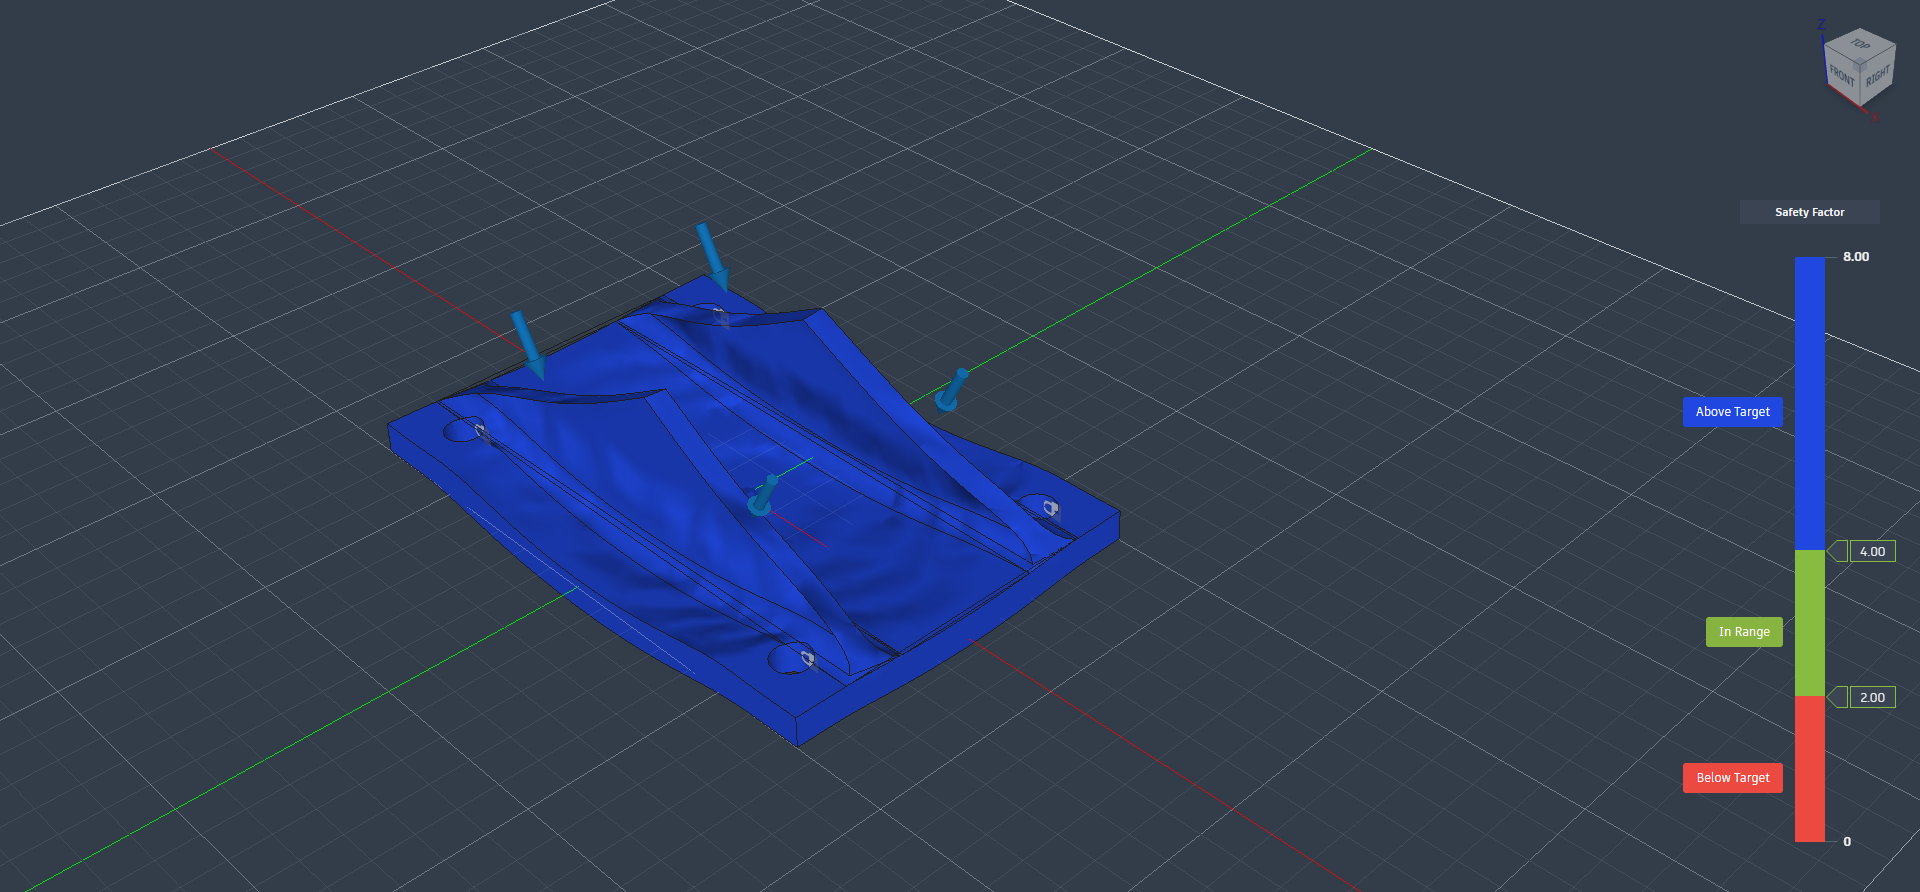
\includegraphics[width=\textwidth]{./images/fusion/study_1_03.png}
\caption*{(a) Study~1 factor-of-safety plot}
\end{minipage}

\vspace{0.25cm}
\begin{minipage}{0.88\textwidth}
\centering
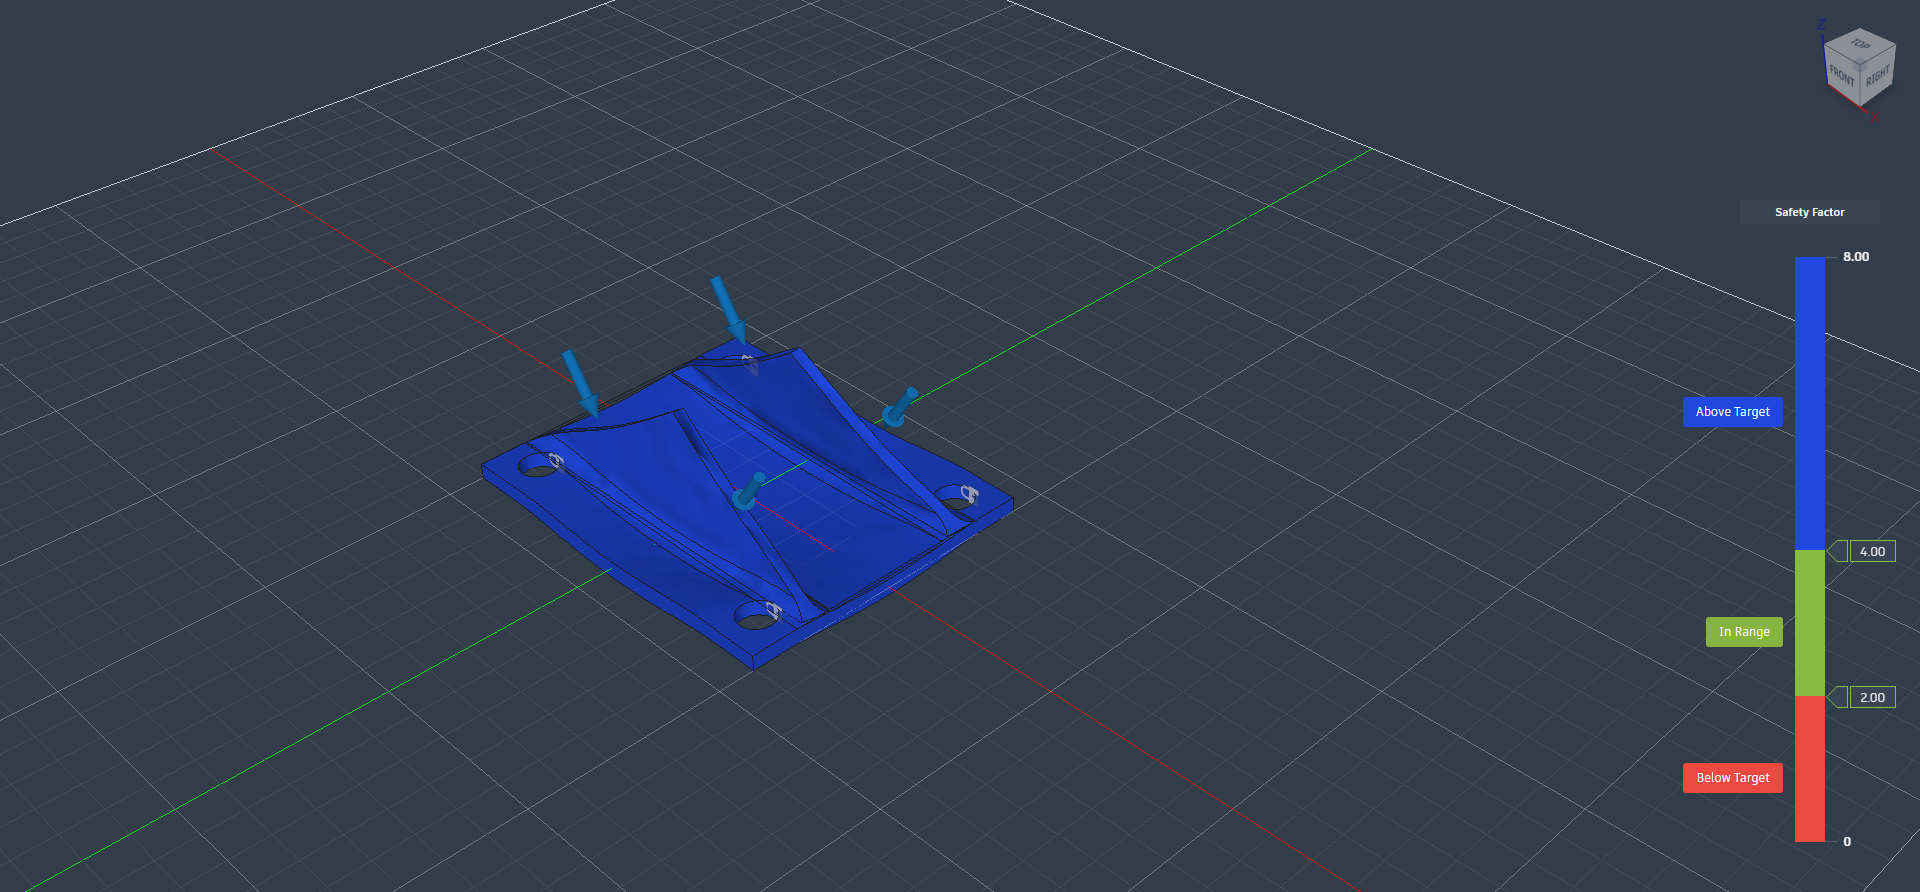
\includegraphics[width=\textwidth]{./images/fusion/study_2_05.png}
\caption*{(b) Study~2 factor-of-safety plot}
\end{minipage}
\caption{Factor-of-safety plots from Studies~1 and~2. The common display cap
of 8 masks the much larger reported values produced by the incorrect
newton-scale loading.}
\label{fig:bracket-fos-comparison}
\end{figure}

The von Mises plots in Figure~\ref{fig:bracket-stress-comparison} show higher
stress around the mounting-hole edges, rib roots, and load-introduction
regions. These locations are consistent with the expected load path and
identify where local mesh refinement and more realistic bolt/contact modelling
would be required. The maxima of 0.016~MPa and 0.026~MPa cannot be used for
acceptance because neither study represents the design load.

\begin{figure}[H]
\centering
\begin{minipage}{0.88\textwidth}
\centering
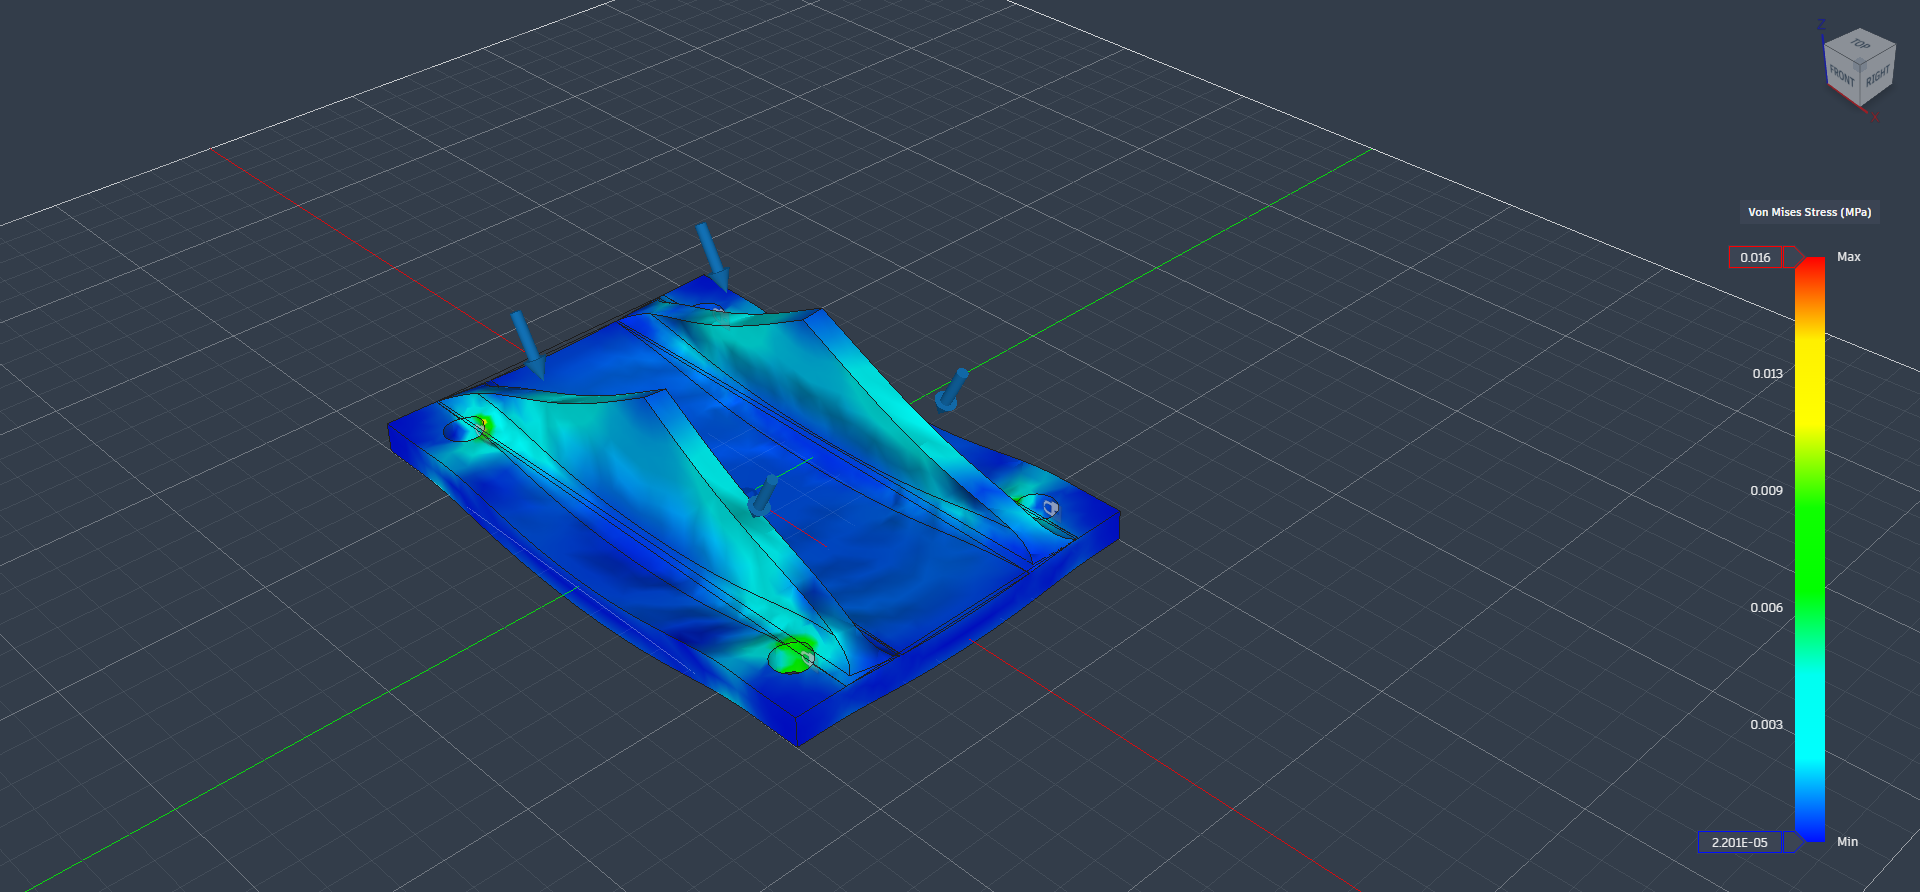
\includegraphics[width=\textwidth]{./images/fusion/study_1_05.png}
\caption*{(a) Study~1 von Mises stress}
\end{minipage}

\vspace{0.25cm}
\begin{minipage}{0.88\textwidth}
\centering
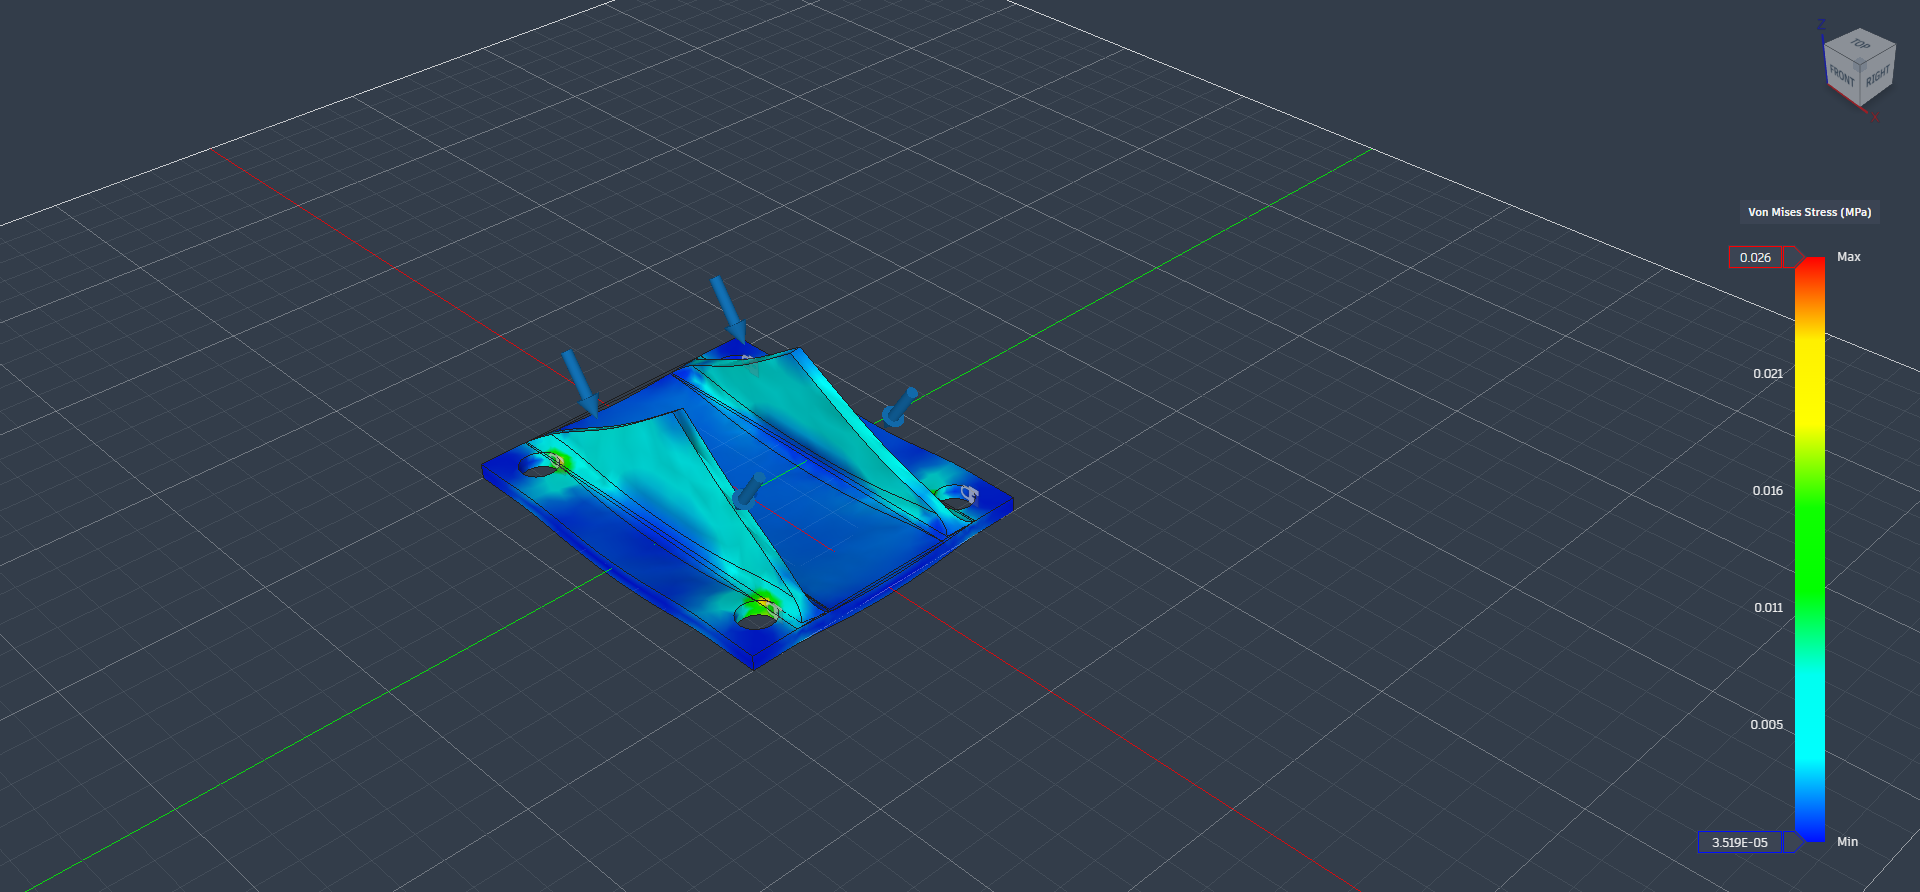
\includegraphics[width=\textwidth]{./images/fusion/study_2_07.png}
\caption*{(b) Study~2 von Mises stress}
\end{minipage}
\caption{Von Mises stress distributions from the two exploratory studies.
Only the qualitative locations are retained as useful evidence.}
\label{fig:bracket-stress-comparison}
\end{figure}

Figure~\ref{fig:bracket-displacement-comparison} shows minimum displacement
near the constrained mounting holes and larger movement across the
unconstrained plate and rib regions. This is qualitatively consistent with the
selected supports. The two maximum values remain several orders of magnitude
below the analytical screening displacement because the applied study loads
were several orders of magnitude too small. No calibration conclusion can
therefore be drawn from the apparent difference between the analytical and
solver responses.

\begin{figure}[H]
\centering
\begin{minipage}{0.88\textwidth}
\centering
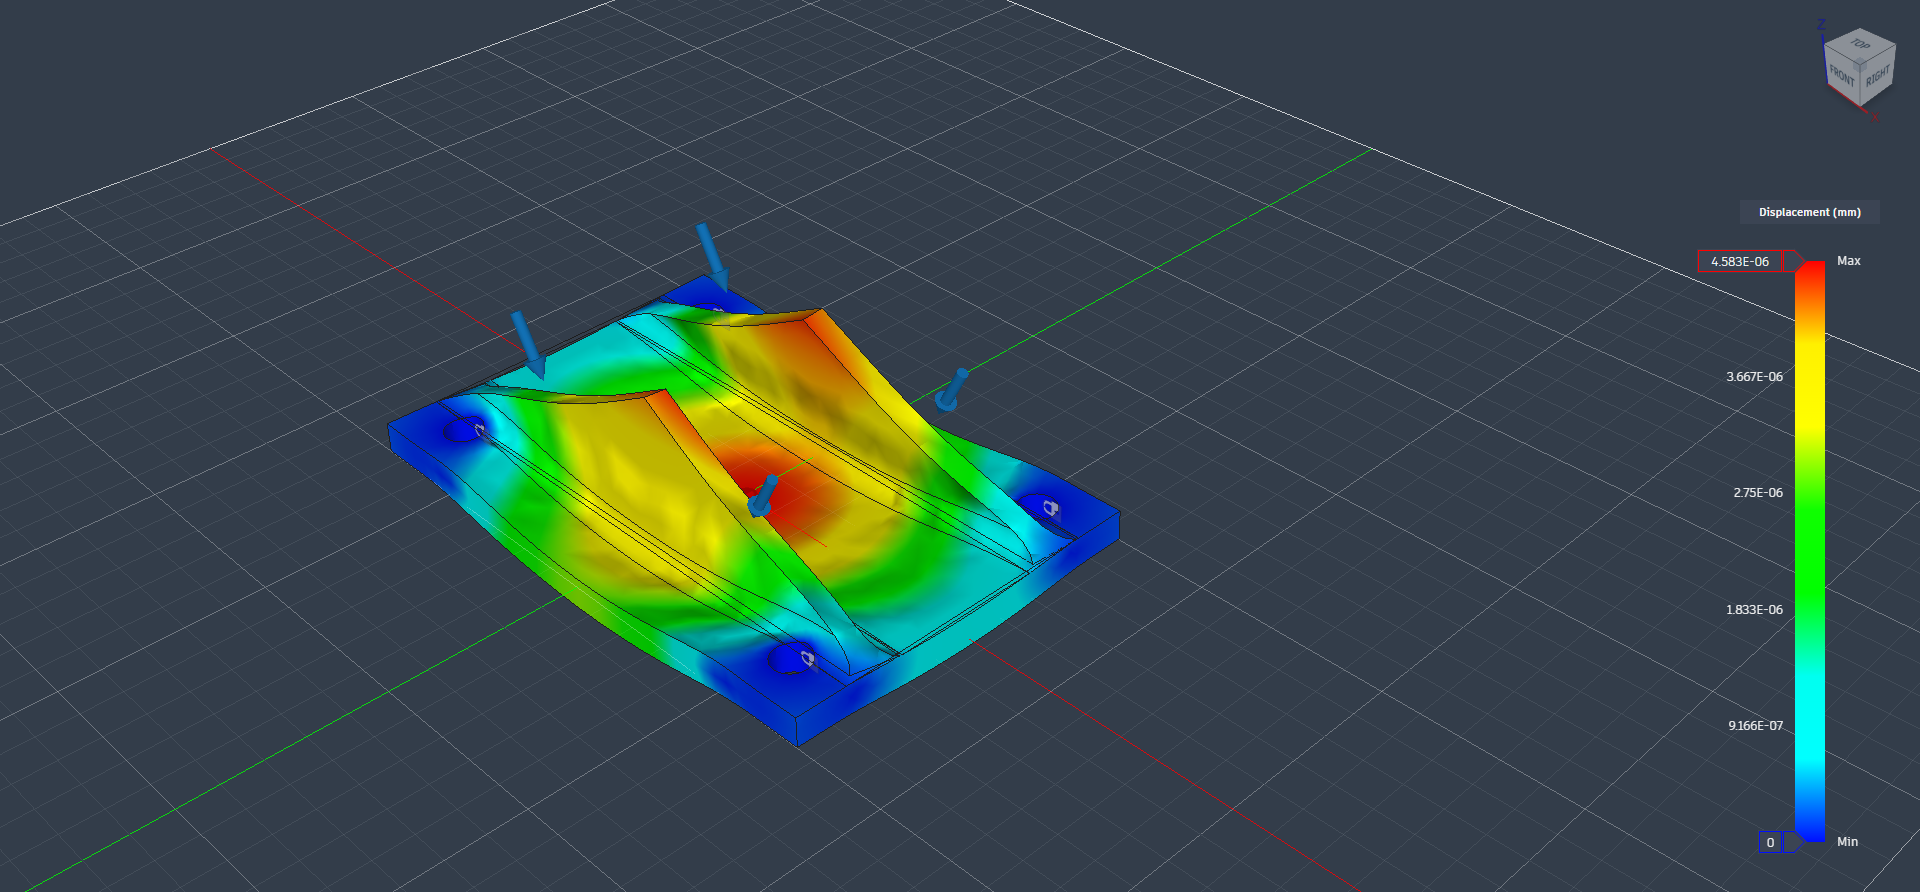
\includegraphics[width=\textwidth]{./images/fusion/study_1_08.png}
\caption*{(a) Study~1 total displacement}
\end{minipage}

\vspace{0.25cm}
\begin{minipage}{0.88\textwidth}
\centering
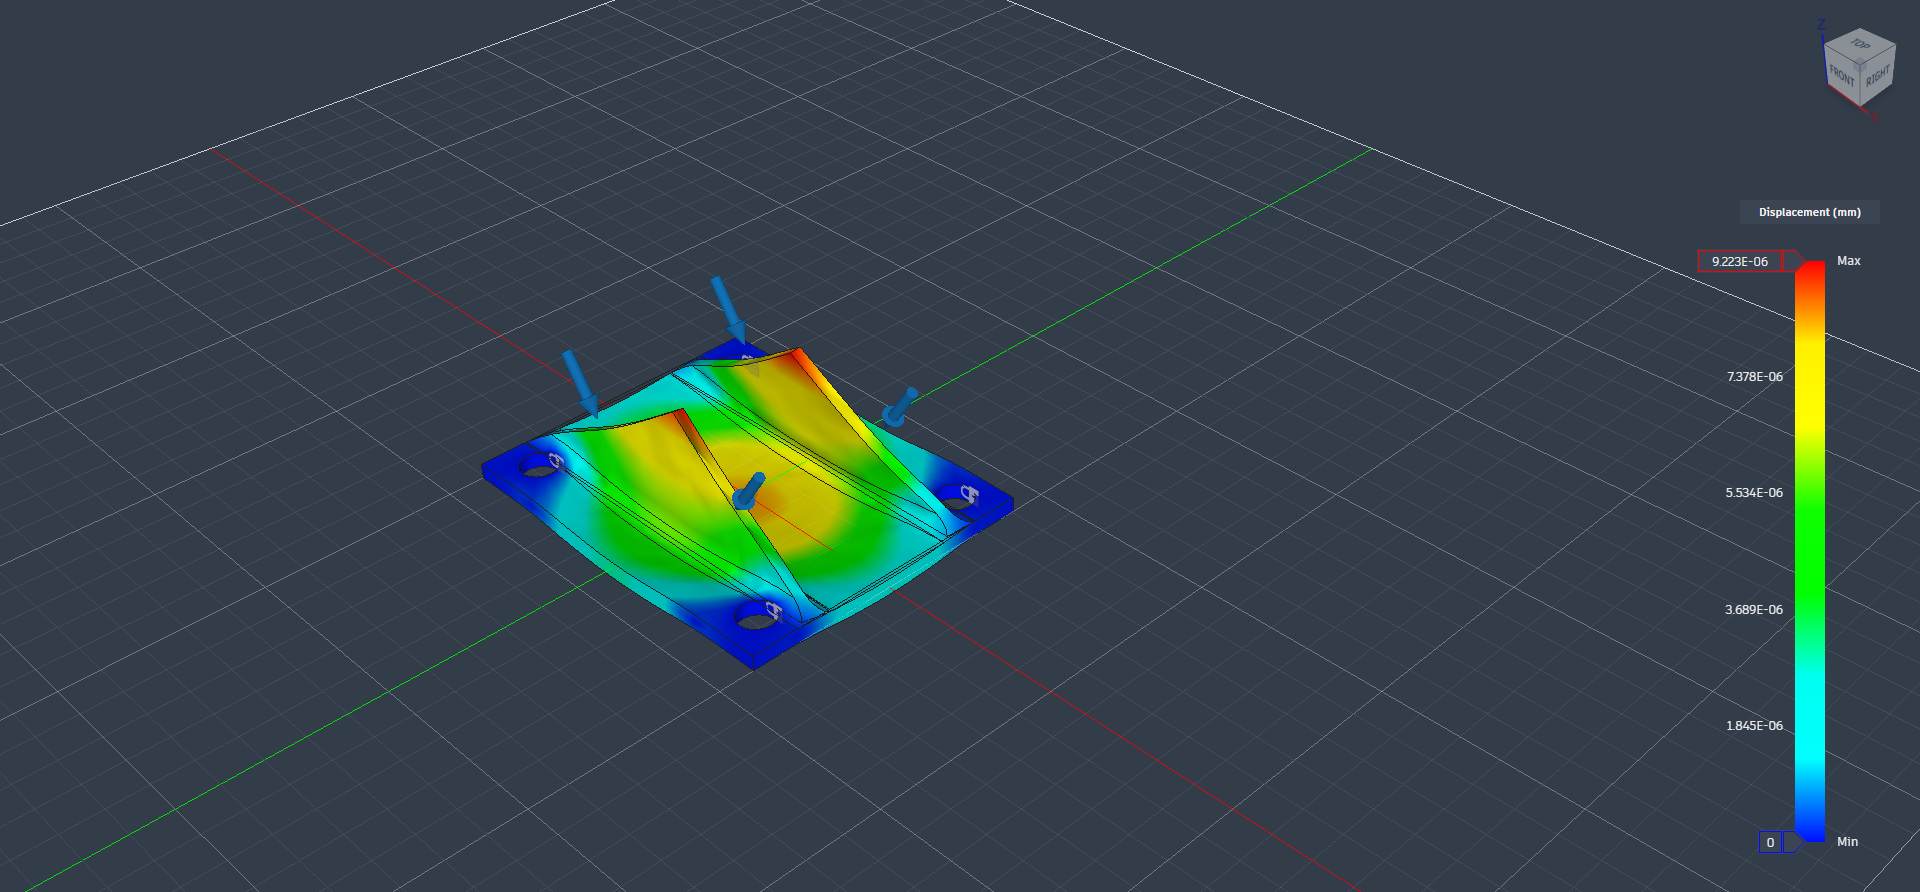
\includegraphics[width=\textwidth]{./images/fusion/study_2_09.png}
\caption*{(b) Study~2 total displacement}
\end{minipage}
\caption{Total-displacement distributions from Studies~1 and~2. The spatial
patterns are informative, but the magnitudes are invalid for the project load.}
\label{fig:bracket-displacement-comparison}
\end{figure}

The bracket studies therefore remain valuable as audit evidence. They confirm
that the native geometry reached the Simulation workspace, show the intended
support and load regions, and reveal plausible qualitative response
locations. They also demonstrate that solver completion is not an acceptance
criterion. A corrected 1472~N study must verify material data, direction,
reaction balance, contact assumptions, local mesh refinement, and convergence
before stress, factor of safety, or displacement is compared with the
analytical finalist.

\clearpage
\section{Discussion}
\label{sec:results-discussion}

\subsection{Achievement of the Project Objectives}
\label{sec:objective-achievement}

\begin{longtable}{
    >{\raggedright\arraybackslash}p{0.08\textwidth}
    >{\raggedright\arraybackslash}p{0.48\textwidth}
    >{\raggedright\arraybackslash}p{0.34\textwidth}}
\caption{Achievement of the specific objectives}
\label{tab:objective-achievement}\\
\toprule
\textbf{No.} & \textbf{Objective outcome} & \textbf{Status}\\
\midrule
\endfirsthead
\toprule
\textbf{No.} & \textbf{Objective outcome} & \textbf{Status}\\
\midrule
\endhead
\bottomrule
\endfoot
1 & Unit-aware parameter spaces, materials, loads, constraints, screening
models, and boundary roles were defined for all three components. &
Achieved for analytical screening and CAD preparation.\\
2 & Each part completed 60 seeded LHS evaluations and three bounded
Nelder--Mead starts; failed evaluations remained controlled. &
Achieved.\\
3 & Native Fusion geometry, physical properties, exchange artifacts, and
semantic boundary evidence were generated. &
Achieved for serialized CAD requests.\\
4 & Baseline plus 20-vector CAD sweeps and baseline/finalist validation sets
were completed. &
Achieved, with the stabilizer outer-process timeout disclosed.\\
5 & Lower-mass analytical finalists were selected and their mass estimates
were compared with native CAD. &
Achieved as screening evidence; all mass differences were within 3.8\%.\\
6 & The bracket proof of concept reached manual Static Stress review, and the
remaining evidence required for design acceptance was identified. &
Partly achieved; both exploratory solver studies were rejected and a corrected
1472~N study remains required.\\
\end{longtable}

\subsection{Limitations of the Results}
\label{sec:results-limitations}

The analytical models are intentionally first order. They use simplified load
paths, nominal section properties, and approximate concentration factors. The
reported constraints include yield-based factor of safety and displacement
only.

The search used a finite sample and three local starts. A different seed,
start, penalty, bound, or model can produce a different candidate. Several
finalists lie near lower bounds, so the selected bounds strongly influence the
result.

The CAD sweeps verify sampled geometry, not the full continuous design space.
They also do not check manufacturing drawings, tolerances, weld access, or
assembly.

The manual FEA evidence is incomplete. The available bracket report has an
incorrect load and cannot validate stress or displacement. Padeye and
stabilizer solver campaigns remain future work. No physical tests were
performed.

\subsection{Engineering Interpretation}

The results support the central workflow claim: inexpensive analytical
evaluation can reduce a large design set to a small group of traceable
candidates, and native CAD can check geometry and mass before manual FEA.
They do not support certification or fabrication.

The most important result is not the largest percentage reduction. It is the
separation of claims. The system recorded analytical predictions, returned
partial CAD responses without solver values, disclosed the stabilizer timeout,
and rejected a completed Fusion report after finding the wrong load. This
behavior is consistent with an auditable engineering workflow.

\chapter{Project Workplan}
\label{chap:workplan}

This chapter presents the project schedule from September 2026 to March 2027.
The workplan groups the study into research and engineering definition,
implementation, verification, and reporting activities. Detailed technical
methods and findings are presented in Chapters~\ref{chap:methodology} and
\ref{chap:results}, respectively.

\section{Project Schedule}
\label{sec:workplan}

The workplan spans seven months. September and October establish the research
basis, engineering definitions, and bracket proof of concept. November and
December develop the design-space search, result records, and multi-part
architecture. January and February focus on native CAD generation,
verification, validation preparation, and analysis of the results. March is
reserved for final reporting, demonstration, corrections, and submission.

The Fusion proof of concept provides the principal technical decision point.
Because the public API does not provide dependable automated control of the
Static Stress workspace, the workflow retains analytical optimization and
native CAD generation while treating solver assessment as a controlled manual
activity. Figure~\ref{fig:gantt} summarizes the sequence. Documentation and
report writing overlap the engineering work because assumptions, decisions,
and evidence are recorded throughout the project.

\begin{figure}[H]
\centering
\begin{ganttchart}[
    hgrid,
    vgrid,
    x unit=1.05cm,
    y unit title=0.62cm,
    y unit chart=0.55cm,
    title label font=\bfseries\scriptsize,
    bar label font=\scriptsize,
    group label font=\bfseries\scriptsize,
    milestone label font=\scriptsize,
    bar/.append style={fill=nemoblue!35,draw=nemoblue},
    group/.append style={fill=nemoteal!35,draw=nemoteal},
    milestone/.append style={fill=nemoorange,draw=nemoorange}
]{1}{7}
\gantttitle{2026}{4}\gantttitle{2027}{3}\\
\gantttitle{Sep}{1}
\gantttitle{Oct}{1}
\gantttitle{Nov}{1}
\gantttitle{Dec}{1}
\gantttitle{Jan}{1}
\gantttitle{Feb}{1}
\gantttitle{Mar}{1}\\

\ganttgroup{Research and definition}{1}{2}\\
\ganttbar{Scope and literature}{1}{2}\\
\ganttbar{Bracket model}{1}{2}\\

\ganttgroup{Implementation}{2}{5}\\
\ganttbar{Fusion proof of concept}{2}{3}\\
\ganttbar{Sampling and optimization}{3}{4}\\
\ganttbar{Padeye and stabilizer}{4}{5}\\
\ganttbar{Native CAD generators}{5}{5}\\

\ganttgroup{Verification and reporting}{5}{7}\\
\ganttbar{Tests and CAD sweeps}{5}{6}\\
\ganttbar{FEA preparation and results}{6}{6}\\
\ganttbar{Documentation and report}{1}{7}\\
\ganttbar{Final QA and demonstration}{7}{7}\\
\ganttmilestone{Submission}{7}
\end{ganttchart}
\caption{Project workplan for September 2026 to March 2027}
\label{fig:gantt}
\end{figure}

\section{Workplan Review}
\label{sec:workplan-review}

The schedule allows analytical development and CAD verification to proceed
before the final simulation review. This sequencing limits the number of
candidates that require higher-fidelity assessment. It also provides time in
March for resolving report corrections and presenting the evidence generated
by the project. Where Fusion-dependent work is delayed, the analytical models,
recorded CAD requests, and validation packages preserve progress and allow the
affected activity to resume without repeating the full design-space search.

\chapter{Project Budget}
\label{chap:budget}

This chapter presents the direct-cash budget and the in-kind resources used by
the project. The work is planned around existing computing facilities,
educational software access, open-source tools, and digital submission.
Consequently, the direct-cash budget is zero, although the project still
depends on material institutional and personal resources.

\section{Direct-Cash Budget}
\label{sec:budget}

No equipment, commercial software, cloud computation, data, printing, travel,
fabrication, or testing service is purchased from project funds.
Table~\ref{tab:cash-budget} summarizes the resulting budget.

\begin{table}[H]
\centering
\caption{Direct-cash project budget}
\label{tab:cash-budget}
\small
\begin{tabularx}{\textwidth}{
    >{\raggedright\arraybackslash}p{0.23\textwidth}
    >{\raggedright\arraybackslash}X
    >{\centering\arraybackslash}p{0.15\textwidth}}
\toprule
\textbf{Category} & \textbf{Basis for zero direct expenditure} &
\textbf{Budget (KES)}\\
\midrule
Development hardware &
Existing personal or university computers are used. No computer or upgrade is
purchased for the project. & 0\\[0.35em]

CAD and simulation software &
Autodesk educational access is used. No commercial licence is purchased from
project funds. & 0\\[0.35em]

Python and report software &
Python, project libraries, Git, and the LaTeX toolchain are available without
direct project charges. & 0\\[0.35em]

Cloud computing and storage &
Computation and working data remain local or use existing remote access. No
paid cloud service is purchased. & 0\\[0.35em]

Internet and electricity &
Existing personal or university services support the work. No separate project
subscription or utility purchase is budgeted. & 0\\[0.35em]

Printing, travel, and communication &
The report is prepared for digital submission. No project-specific printing,
travel, or communication expense is charged. & 0\\[0.35em]

Prototype fabrication and testing &
No physical component or paid laboratory test is included in the project
scope. & 0\\[0.35em]

Contingency &
The contingency consists of schedule margin and scope control rather than a
cash allocation. & 0\\
\midrule
\textbf{Total direct-cash budget} & & \textbf{0}\\
\bottomrule
\end{tabularx}
\end{table}

\section{In-Kind Resources}
\label{sec:in-kind-resources}

A zero direct-cash budget does not imply that the project uses no resources.
Existing computers, Autodesk educational access, internet, electricity,
supervision, and student labour are in-kind inputs. Table~\ref{tab:in-kind}
records these resources without assigning unsupported monetary values.

\begin{table}[H]
\centering
\caption{In-kind resources used but not monetized}
\label{tab:in-kind}
\small
\begin{tabularx}{\textwidth}{
    >{\raggedright\arraybackslash}p{0.25\textwidth}
    >{\raggedright\arraybackslash}X
    >{\raggedright\arraybackslash}X}
\toprule
\textbf{Resource} & \textbf{Provision basis} & \textbf{Project use}\\
\midrule
Computers & Existing personal or university access &
Python development, testing, Fusion CAD, simulation, report compilation, and
demonstration.\\

Autodesk Fusion & Educational entitlement &
Native CAD generation, physical-property evaluation, STEP export, and Static
Stress preparation.\\

Open-source software & Public software licences &
Optimization, testing, data recording, visualization, version control, and
report production.\\

Internet and electricity & Existing personal or institutional access &
Research, reference consultation, source synchronization, and software
operation.\\

Student labour and supervision & Academic project activity &
Engineering definition, implementation, review, testing, analysis,
documentation, and presentation preparation.\\
\bottomrule
\end{tabularx}
\end{table}

\section{Budget Control}
\label{sec:budget-control}

The project architecture supports the zero direct-cash budget by using
analytical equations for the broad design-space search and reserving manual FEA
review for a small number of candidates. The in-application Fusion API and
local data exchange avoid paid cloud automation, while open-source Python tools
and digital reporting avoid additional software and printing costs.

Prototype fabrication and paid testing remain outside the present academic
scope; they are not treated as unnecessary. Progression towards a
service-ready design requires a separate budget for material certification,
fabrication, inspection, instrumentation, proof loading, calibrated FEA, and
any required hydrodynamic testing.

\chapter{Conclusions and Recommendations}
\label{chap:conclusion}

This chapter presents the conclusions supported by the analytical, CAD, and
bracket-study evidence. It also states the limitations of the work and the
validation required before any candidate can progress toward manufacture or
service.

\section{Conclusions}
\label{sec:overall-conclusion}

The study developed and evaluated an auditable, resource-conscious workflow
for the parameterized mass optimization of three marine structural component
archetypes. The same overall process represented a bracket, padeye, and
stabilizer while allowing each component to retain its own variables,
material, load, analytical formulation, CAD generator, and boundary roles.
This supports the use of a shared part-aware architecture within the reported
scope.

Seeded Latin-hypercube exploration and three bounded Nelder--Mead starts
identified lower-mass candidates that satisfied the implemented analytical
factor-of-safety and displacement criteria. The selected screening reductions
were 72.9\% for the bracket, 59.9\% for the padeye, and 27.2\% for the
stabilizer relative to their configured baselines. Multiple starts improved
the best feasible mass for every part. These values describe the best
feasible designs found within the declared parameterized searches; they do not
prove global optimality or service-ready weight savings.

Native Fusion generation remained usable across the seeded CAD campaigns. The
bracket and padeye completed all 21 baseline-plus-sample cases. The stabilizer
created all 21 artifact sets, although the outer process timed out while
reading the final response. Analytical and native-CAD mass differed by no more
than 3.8\% for the six baseline and finalist comparisons. This agreement
supports the volume models for early mass ranking, but it does not validate
stress or displacement.

The two bracket Static Stress studies provide the clearest lesson about
evidence quality. Their images identify the geometry, mounting-hole supports,
rib-face loading, and qualitative response regions. Study~2 also records the
mesh and boundary setup more clearly than Study~1. Nevertheless, Study~2 used
1.472~N instead of the intended 1472~N, while Study~1 did not provide a
complete traceable load definition and reported only a 1.298~N support
reaction. The numerical stress, factor of safety, and displacement values from
both studies were therefore rejected.

The principal outcome is a traceable method for reducing a large design set,
checking native geometry and mass, and preparing a small candidate set for
disciplined validation. The study does not establish structural
qualification, fabrication readiness, or service safety.

\section{Achievement of the Objectives}
\label{sec:aim-achievement}

The aim was achieved at the level of workflow development, analytical
screening, native-CAD verification, and validation preparation. Unit-aware
engineering definitions and screening models were completed for all three
parts; the sampling and multi-start searches were executed; invalid
evaluations were contained; native geometry, physical properties, exchange
artifacts, and boundary evidence were produced; and analytical-to-CAD mass
agreement was assessed. Table~\ref{tab:objective-achievement} records the
status of each specific objective.

The aim was only partly achieved at the structural-validation level. The
bracket reached manual FEA review, but the two exploratory studies did not use
a sufficiently traceable and correct design load. Corrected, mesh-converged
FEA has not yet been completed for the selected bracket, padeye, or stabilizer
candidates.

\section{Limitations}
\label{sec:conclusion-limitations}

The analytical models are first-order representations of selected load paths.
They omit detailed fastener and weld behaviour, nonlinear contact,
three-dimensional local stress, fatigue, buckling, corrosion, vibration,
impact, and other component-specific service effects. The stabilizer load is a
prescribed structural envelope rather than a pressure field derived from CFD,
model tests, or measurements.

The search uses a finite 60-point sample, three local starts, fixed bounds, and
a penalty objective. A different seed, model, bound, or constraint strategy
could produce a different finalist. Several selected parameters lie near
their lower bounds, which indicates that manufacturing limits and omitted
failure modes can materially affect the result.

The CAD sweeps cover seeded design vectors rather than every point in the
continuous space. They verify geometry, mass, artifacts, and boundary
identification, but do not verify drawings, tolerances, assembly, weld access,
or manufacturability. No acceptable finalist FEA or physical test result is
available.

\section{Recommendations}
\label{sec:recommendations}

\begin{enumerate}
    \item Recreate the bracket study with a verified total load of 1472~N,
    confirm its coordinate direction, keep force per entity disabled, and
    demonstrate reaction balance. Compare the baseline, lightest finalist, and
    conservative backup candidates using at least three systematically refined
    meshes.
    \item Replace the rigid hole constraint with more realistic bolt, bearing,
    contact, and preload representations when these effects influence the
    bracket decision. Assess local plate behaviour, rib-root and weld stress,
    fatigue, corrosion allowance, fabrication tolerance, and supporting
    structure.
    \item Validate the padeye under the governing lifting standard and load
    combinations. Begin with a distributed bearing model and progress to a
    separate pin with clearance and nonlinear contact where required. Check
    net section, bearing, shear-out, lug root, gussets, welds, fatigue,
    inspection, and proof-load requirements.
    \item Derive stabilizer pressure cases from an accepted hydrodynamic method,
    CFD, model tests, or measurements. Include positive and negative loading,
    torsion, root and spar stresses, skin-panel buckling, fatigue, corrosion,
    actuator interaction, vibration, and tip displacement.
    \item Compare corrected FEA responses with the analytical predictions at
    identical candidate geometries and loads. Any calibration should use
    separate fitting and checking candidates and remain limited to the
    supported parameter range.
    \item Treat the lightest analytical row as one candidate rather than the
    automatic design choice. Material certification, applicable codes,
    uncertainty, fabrication, inspection, physical testing where required,
    and qualified engineering review must precede acceptance.
\end{enumerate}

\section{Future Work}
\label{sec:future-research}

Future development can introduce a formal multi-fidelity strategy in which
selected FEA results correct analytical bias or support a surrogate model with
explicit uncertainty. Reliability-based optimization can then represent
variability in loads, material properties, fabrication dimensions, corrosion,
and modelling error.

The search can also be extended from single-objective mass minimization to a
multi-objective formulation that includes fabrication cost, fatigue damage,
displacement, or embodied carbon. Manufacturing-aware constraints should
represent minimum gauges, available stock sizes, tool and inspection access,
weld size, bend radii, and tolerance sensitivity.

For the individual components, the bracket can be extended to equipment
vibration and foundation flexibility, the padeye to lifting-operation load
angles and proof testing, and the stabilizer to coupled hydrodynamic and
structural loading. Each extension should preserve the distinction between a
screening prediction, a CAD property, a solver result, and a validated design.


\label{page:main-end}
\clearpage

% ==============================================================================
% REFERENCES AND APPENDICES
% ==============================================================================

\bibliographystyle{IEEEtran}
\bibliography{references}

\appendix
\chapter{Reproduction and Validation Material}
\label{chap:appendices}

\section{Fresh-Start Command-Prompt Procedure}
\label{app:fresh-start}

The following procedure uses Windows Command Prompt. It does not require
PowerShell.

\begin{enumerate}
    \item Open Command Prompt.
    \item Change to the repository:
\begin{lstlisting}[language={},caption={Open the NEMO repository}]
cd /d C:\Users\muigu\Documents\Projects\NEMO
\end{lstlisting}
    \item Create or update the project environment:
\begin{lstlisting}[language={},caption={Set up the project}]
build.bat setup
\end{lstlisting}
    \item Run the offline checks:
\begin{lstlisting}[language={},caption={Run offline verification}]
build.bat check
\end{lstlisting}
    \item List the registered parts:
\begin{lstlisting}[language={},caption={List the registered components}]
.venv\Scripts\nemo.exe parts
\end{lstlisting}
    \item Evaluate the three baselines:
\begin{lstlisting}[language={},caption={Evaluate the analytical baselines}]
.venv\Scripts\nemo.exe evaluate --part bracket
.venv\Scripts\nemo.exe evaluate --part padeye
.venv\Scripts\nemo.exe evaluate --part stabilizer
\end{lstlisting}
\end{enumerate}

\section{Bracket Proof-of-Concept Procedure}
\label{app:bracket-poc}

\begin{enumerate}
    \item Start Autodesk Fusion.
    \item Open \emph{Utilities}, then \emph{Scripts and Add-Ins}.
    \item Select and start NEMOBridge.
    \item If a bracket opens automatically, leave it available. NEMOBridge can
    load or create the demonstration design during startup.
    \item Open Command Prompt and change to the repository.
    \item Run:
\begin{lstlisting}[language={},caption={Run the preserved bracket proof of concept}]
cd /d C:\Users\muigu\Documents\Projects\NEMO
.venv\Scripts\python.exe demos\bracket-proof-of-concept\manual_fusion_handshake.py
\end{lstlisting}
    \item Return to Fusion and inspect the regenerated bracket.
    \item For the complete manual study, follow
    Section~\ref{sec:bracket-poc-method}.
\end{enumerate}

\section{Schema-Version-2 Request Example}
\label{app:schema-request}

\begin{lstlisting}[language=Python,caption={Illustrative bracket CAD request},
label={lst:request-example}]
{
  "schema_version": 2,
  "part_id": "bracket",
  "run_id": "demo_bracket",
  "iteration": 0,
  "mode": "fusion_cad",
  "parameters": {
    "baseplate_length": 150.0,
    "baseplate_width": 100.0,
    "baseplate_thickness": 8.0,
    "rib_height": 40.0,
    "rib_thickness": 6.0,
    "fillet_radius": 5.0
  },
  "artifact_formats": ["step", "boundary_tags"]
}
\end{lstlisting}

\section{CAD-Only Response Example}
\label{app:schema-response}

\begin{lstlisting}[language=Python,caption={Illustrative partial CAD response},
label={lst:response-example}]
{
  "schema_version": 2,
  "part_id": "bracket",
  "run_id": "demo_bracket",
  "iteration": 0,
  "status": "partial",
  "metrics": {
    "mass_kg": 0.4228127502,
    "volume_m3": 0.0001565973,
    "max_stress_mpa": null,
    "factor_of_safety": null,
    "max_deflection_mm": null,
    "objective_value": null
  },
  "artifacts": {
    "step": "...\\bracket_0000.step",
    "boundary_tags": "...\\bracket_0000.boundaries.json"
  },
  "error": "Native CAD generation and mass extraction completed.
            Static-stress results require manual Fusion validation."
}
\end{lstlisting}

The partial status is intentional. It prevents a CAD success from being
interpreted as an FEA success.

\section{Selected Finalist Parameters}
\label{app:finalist-parameters}

\begin{table}[H]
\centering
\caption{Selected bracket finalist parameters}
\label{tab:app-bracket-finalist}
\begin{tabularx}{\textwidth}{Xr}
\toprule
\textbf{Parameter} & \textbf{Value (mm)}\\
\midrule
Baseplate length & 100.0328\\
Baseplate width & 80.9380\\
Baseplate thickness & 4.0429\\
Rib height & 33.2576\\
Rib thickness & 3.0000\\
Fillet radius & 3.5308\\
\bottomrule
\end{tabularx}
\end{table}

\begin{table}[H]
\centering
\caption{Selected padeye finalist parameters}
\label{tab:app-padeye-finalist}
\begin{tabularx}{\textwidth}{Xr}
\toprule
\textbf{Parameter} & \textbf{Value (mm)}\\
\midrule
Base length & 220.3878\\
Base width & 150.4654\\
Base thickness & 8.0484\\
Lug height & 141.7256\\
Lug thickness & 12.1613\\
Neck width & 80.0000\\
Gusset height & 70.0000\\
Gusset thickness & 6.2101\\
Fillet radius & 25.0000\\
\bottomrule
\end{tabularx}
\end{table}

\begin{table}[H]
\centering
\caption{Selected stabilizer finalist parameters}
\label{tab:app-stabilizer-finalist}
\begin{tabularx}{\textwidth}{Xlr}
\toprule
\textbf{Parameter} & \textbf{Unit} & \textbf{Value}\\
\midrule
Skin thickness & mm & 4.0106\\
Front spar position & \% chord & 25.0000\\
Rear spar position & \% chord & 72.0000\\
Front spar thickness & mm & 7.8522\\
Rear spar thickness & mm & 6.5297\\
Rib thickness & mm & 5.6971\\
Root insert length & mm & 221.4762\\
Root insert thickness & mm & 13.6624\\
Root fillet radius & mm & 18.3273\\
\bottomrule
\end{tabularx}
\end{table}

\section{Manual FEA Validation Record}
\label{app:fea-record}

Each baseline and finalist FEA record should contain the fields in
Table~\ref{tab:app-fea-checklist}.

\begin{longtable}{p{0.25\textwidth}p{0.65\textwidth}}
\caption{Minimum manual FEA validation checklist}
\label{tab:app-fea-checklist}\\
\toprule
\textbf{Record item} & \textbf{Required evidence}\\
\midrule
\endfirsthead
\toprule
\textbf{Record item} & \textbf{Required evidence}\\
\midrule
\endhead
\bottomrule
\endfoot
Candidate identity &
Part identifier, candidate identifier, source run, iteration, parameter table,
schema version, and generator version.\\

Geometry &
Native CAD screenshot, connected-body count, volume, mass, and STEP path.\\

Material &
Name, density, Young's modulus, Poisson ratio, yield strength, and source.\\

Load &
Magnitude, unit, derivation, direction, selected faces, distribution, and
force-per-entity state.\\

Support &
Constraint type, selected faces, physical interpretation, and screenshot.\\

Contact &
Contact type, interfaces, assumptions, and any nonlinear settings.\\

Mesh &
Element type and order, global size, local sizes, growth control, node count,
element count, and screenshot.\\

Equilibrium &
Applied-load vector, support-reaction vector, imbalance, and percentage
difference.\\

Stress &
Maximum von Mises stress, location, stable nearby monitored stress, and
contour screenshot.\\

Factor of safety &
Minimum value, location, yield definition, and contour screenshot.\\

Displacement &
Maximum magnitude, monitored displacement, direction, and location.\\

Convergence &
At least three meshes, same monitored locations, result changes, and selected
mesh justification.\\

Acceptance &
FOS and displacement pass/fail, local failure-mode checks, limitations, and
engineering disposition.\\
\end{longtable}

\section{Bracket Corrected-Study Record Template}
\label{app:bracket-study-template}

\begin{table}[H]
\centering
\caption{Bracket Static Stress input record}
\label{tab:app-bracket-input}
\begin{tabularx}{\textwidth}{p{0.30\textwidth}X}
\toprule
\textbf{Field} & \textbf{Required entry}\\
\midrule
Material & Project Aluminum 6061-T6 properties\\
Analytical load & 1471.5~N\\
Fusion force input & \textbf{1472 N total}\\
Force per entity & Off\\
Loaded faces & Four upper sloping rib faces\\
Load direction & Downward in the declared study coordinate system\\
Supports & Four mounting-hole cylindrical faces\\
Element order & Parabolic\\
Local refinements & Mounting holes and rib-root fillets\\
Reaction target & Approximately 1472~N opposite the applied direction\\
Constraint checks & FOS $\geq2.5$ and displacement $\leq0.5$~mm\\
\bottomrule
\end{tabularx}
\end{table}

\section{Mesh-Convergence Template}
\label{app:mesh-template}

\begin{table}[H]
\centering
\caption{Mesh-convergence recording template}
\label{tab:app-mesh-template}
\small
\resizebox{\textwidth}{!}{%
\begin{tabular}{crrrrr}
\toprule
\textbf{Mesh} & \textbf{Nodes} & \textbf{Elements} &
\textbf{Peak stress (MPa)} & \textbf{Monitored stress (MPa)} &
\textbf{Displacement (mm)}\\
\midrule
1 & & & & &\\
2 & & & & &\\
3 & & & & &\\
4 & & & & &\\
\bottomrule
\end{tabular}%
}
\end{table}

Mesh 1 is the coarse reference, meshes 2 and 3 are successive refinements, and
mesh 4 is an optional confirmation. The monitored stress must use the same
geometric region on every mesh. A moving global maximum is not a valid
convergence quantity when it moves between unrelated singular edges.

\section{Stabilizer Pressure-Band Calculation}
\label{app:pressure-bands}

Let the unnormalized weights be

\begin{equation}
\mathbf{w}=[1.00,\ 0.93,\ 0.75,\ 0.40].
\end{equation}

Their sum is 3.08. The band-force fractions are:

\begin{equation}
\hat{\mathbf{w}}=
[0.324675,\ 0.301948,\ 0.243506,\ 0.129870].
\end{equation}

For the 11\,808~N resultant, the approximate band forces are:

\begin{table}[H]
\centering
\caption{Prescribed stabilizer pressure-band forces}
\label{tab:app-pressure-bands}
\begin{tabular}{crr}
\toprule
\textbf{Band} & \textbf{Normalized fraction} & \textbf{Force (N)}\\
\midrule
1 & 0.324675 & 3833.8\\
2 & 0.301948 & 3565.4\\
3 & 0.243506 & 2875.1\\
4 & 0.129870 & 1533.8\\
\midrule
Total & 1.000000 & 11\,808.0\\
\bottomrule
\end{tabular}
\end{table}

The FEA pressure for a band is its force divided by its selected CAD face area.
The forces are prescribed engineering inputs and are not CFD results.

\section{Evidence Inventory}
\label{app:evidence-inventory}

\begin{longtable}{>{\raggedright\arraybackslash}p{0.34\textwidth}p{0.56\textwidth}}
\caption{Principal repository evidence used in the report}
\label{tab:app-evidence}\\
\toprule
\textbf{Location} & \textbf{Evidence}\\
\midrule
\endfirsthead
\toprule
\textbf{Location} & \textbf{Evidence}\\
\midrule
\endhead
\bottomrule
\endfoot
\path{src/nemo/parts/definitions} &
Authoritative part parameters, units, materials, loads, constraints, fixed
geometry, and boundary roles.\\

\path{src/nemo/parts/analytical.py} &
First-order volume, stress, factor-of-safety, and displacement equations.\\

\path{src/nemo/optimizer.py} &
Scaled bounded Nelder--Mead search and evaluation handling.\\

\path{src/nemo/logger.py} &
Stable one-part-per-log CSV and JSON records.\\

\path{fusion_addin/NEMOBridge} &
Fusion add-in, native generators, artifact export, and boundary selectors.\\

\path{reports/final_20260728_*_validation} &
Baseline and finalist parameters, analytical metrics, Fusion requests, Fusion
responses, and checklists.\\

\path{F360 report/Study Final.html} &
Bracket manual study setup, mesh metadata, result views, and the recorded
1.472~N force error.\\

\path{demos/bracket-proof-of-concept} &
Preserved initial demonstration flow and historical validation material.\\

\path{reports/project-report} &
LaTeX report source, bibliography, extracted images, reproducible chart
script, and compiled PDF.\\
\end{longtable}

\section{Demonstration Sequence}
\label{app:demo-sequence}

A concise defense demonstration can follow this order:

\begin{enumerate}
    \item state the problem and evidence boundary;
    \item show the three part definitions;
    \item evaluate the three analytical baselines;
    \item show the 60-sample and three-start workflow;
    \item compare baseline and finalist mass;
    \item open one stored validation package;
    \item send or replay a bracket CAD request;
    \item show the native bracket, mass, STEP, and boundary metadata;
    \item identify the four support faces and four upper load faces;
    \item explain the 1.472~N error and the corrected 1472~N procedure;
    \item show how padeye and stabilizer roles extend the same architecture;
    \item close with the validation work required before manufacture.
\end{enumerate}

\section{Report Metadata Requiring Confirmation}
\label{app:metadata-placeholders}

The title-page project code remains \code{MR-PRO-26-XX}, and the supervisor is
shown as \code{SUPERVISOR NAME}. These placeholders must be replaced with the
official project code and supervisor name before final institutional
submission.


\end{document}
